\documentclass[pra,
aps,
twocolumn,
superscriptaddress,
groupedaddress,
nofootinbib,
reprint
]{revtex4-1}

% PACKAGES
\usepackage{amsmath,amsfonts, amssymb, amsthm}
\usepackage{bm, bbm, physics, mathtools}
\usepackage{graphicx, subfigure}
\usepackage{xcolor, enumerate}
\usepackage{xifthen, hyperref}
\usepackage[capitalise]{cleveref}

\hypersetup{
	colorlinks=true,  
	linkcolor=blue,   
	citecolor=blue,   
	urlcolor=blue     
}

\newcommand{\crefrangeconjunction}{--}
\creflabelformat{figure}{(#2#1#3)}

% COMMENT NOTATION
\newcommand{\nick}[1]{{\color{red}#1}}
\newcommand{\ddd}[1]{\textcolor{blue}{#1}}

% ENVIRONMENTS
\newtheorem{theorem}{Theorem}
\newtheorem{proposition}[theorem]{Proposition}
\newtheorem{lemma}[theorem]{Lemma}
\newtheorem{definition}[theorem]{Definition}

% REFERENCES
\iffalse
\renewcommand{\eqref}[1]{Eq.~(\ref{#1})}
\newcommand{\figref}[1]{Fig.~(\ref{#1})}
\newcommand{\tabref}[1]{Tab.~(\ref{#1})}
\newcommand{\secref}[1]{Section~(\ref{#1})}
\newcommand{\appref}[1]{Appendix~(\ref{#1})}
\newcommand{\defref}[1]{Definition~\ref{#1}}
\newcommand{\lemref}[1]{Lemma~\ref{#1}}
\newcommand{\thmref}[1]{Theorem~\ref{#1}}
\fi

% SYMBOL DEFINITIONS
\renewcommand{\cal}[1]{\mathcal{#1}}

\newcommand{\reals}{\mathbb{R}}
\newcommand{\id}{\mathbbm{1}}
\newcommand{\idc}{1_{\rm{C}}}
\newcommand{\supf}{\mathfrak{c}}
\renewcommand{\tr}{{\rm{tr}}}
\renewcommand{\det}{{\rm{det}}}
\newcommand{\floor}[1]{\left\lfloor #1 \right\rfloor}
\newcommand{\ent}[2]{S\left( #1 \middle\vert\middle\vert #2 \right)}
\newcommand{\ents}{{\ent{\frac{m}{n}}{p}}}

\def\dummy{\ell}
\def\NN{n}
\def\mmf{i}
\def\nnf{n}
\def\mlt{m}
\def\ii{i}
\def\jj{j}
\def\kk{k}
\def\II{I}
\def\nn{n}
\def\tt{n'}
\def\mm{a}
\def\wp{u}
\def\wn{v}

\newcommand{\too}[1]{^{\otimes #1}}
\newcommand{\noisys}{\rho_{\rm{S}}}
\newcommand{\noisysn}{\rho_{\rm{S}}(\epsilon)^{\otimes \nn}}
\newcommand{\noisysN}{\rho_{\rm{S}}(\epsilon)^{\otimes \NN}}

\newcommand{\spanv}[1]{
    {{\rm{span}}\left\{#1\right\}}
}
\newcommand{\conv}[1]{
    {{\rm{conv}}#1}
}
\newcommand{\orb}[1]{
    {{\rm{orb}}(#1)}
}
\newcommand{\sn}[1]{
    {{\rm{sn}}\left(#1\right)}
}
\newcommand{\mana}[1]{
    {{\rm{mana}}\left(#1\right)}
}
\newcommand{\lc}[2]{
	{{\rm{L}}_{#1|#2}}
}

\newcommand{\bmx}{\bm{x}}
\newcommand{\bmy}{\bm{y}}
\newcommand{\bmz}{\bm{z}}
\newcommand{\bmu}{\bm{u}}
\newcommand{\bmw}{\bm{w}}
\newcommand{\bmo}{\bm{0}}
\newcommand{\bmd}{\bm{d}}
\newcommand{\bma}{\bm{a}}
\newcommand{\bmxi}{\bm{\xi}}
\newcommand{\bmg}{\bm{g}}

\newcommand{\zd}[1][]{
    \ifthenelse{\isempty{#1}}{
    {\mathbb{Z}_d} }{
    {\mathbb{Z}_{#1}}}
}
\newcommand{\hd}[1][]{
    \ifthenelse{\isempty{#1}}{
    {\cal{H}_d} }{
    {\cal{H}_{#1}}}
}
\newcommand{\pd}[1][]{
    \ifthenelse{\isempty{#1}}{
    {\cal{P}_d} }{
    {\cal{P}_{#1}}}
}
\newcommand{\cd}[1][]{
    \ifthenelse{\isempty{#1}}{
    {\cal{C}_d} }{
    {\cal{C}_{#1}}}
}
\newcommand{\spd}[1][]{
    \ifthenelse{\isempty{#1}}{
    {{\rm{Sp}}(2, \zd)} }{
    {{\rm{Sp}}(2, \zd[#1])}}
}
\newcommand{\gp}[1][]{
    \ifthenelse{\isempty{#1}}{
    {\rm{GP}_d} }{
    {\rm{GP}_{#1}}}
}
\newcommand{\stoch}[1][]{
    \ifthenelse{\isempty{#1}}{
    {{\rm{S}}_d(\bmd)} }{
    {{\rm{S}}_d(#1)}}
}
\newcommand{\stochw}[1][]{
    \ifthenelse{\isempty{#1}}{
    {{\rm{S}}_{d^2}(\W{\sigma})} }{
    {{\rm{S}}_{d^2}(#1)}}
}
\makeatletter
\def\W{\@ifnextchar[{\@with}{\@without}}
\def\@with[#1]#2{ 
    {{\rm{W}}_{#2}\left(#1\right)} }
\def\@without#1{ 
    {{\rm{W}}_{#1}} }
\makeatother

\newcommand{\T}{\cal{T}}
\newcommand{\Z}{\cal{Z}}

\newcommand{\C}{\cal{C}}
\newcommand{\E}{\cal{E}}
\newcommand{\J}{\cal{J}}
\newcommand{\R}{\cal{R}}
\newcommand{\D}{\cal{D}}
\newcommand{\F}{\cal{F}}
\renewcommand{\O}{\cal{O}}
\newcommand{\M}{\cal{M}}

\newcommand{\Fmax}{\F_{\rm{max}}}
\newcommand{\Omax}{\O_{\rm{}max}}
\newcommand{\Rmax}{\R_{\rm{}max}}
\newcommand{\Pis}{\Pi_{\rm{s}}}
\newcommand{\Pio}{\Pi_{\rm{o}}}

\newcommand{\cptp}{{\rm{CPTP}}}
\newcommand{\cpos}{{\rm{CP}}}
\newcommand{\so}{{\rm{SO}}}
\newcommand{\stab}{{\rm{STAB}}}
\newcommand{\spo}{{\rm{SPO}}}
\newcommand{\cspo}{{\rm{CSPO}}}
\newcommand{\rcu}{{\rm{RCU}}}
\newcommand{\tho}{{\rm{TO}}}
\newcommand{\cpwp}{{\rm{CPWPO}}}
\newcommand{\ru}{{\rm{RU}}}


\begin{document}
% Write bounds as 1 + ln{}/{} or 1 - (-ln{})/{} ?
% Sec: General resources
% Sec: Lower bounds
% App: D clean-up + d--> r ?

% Figs consistency (esp. figs 3,4,5 and 1,6) + Figure 0 ?

% Eq. numbering in last line always
% UK vs US english
% Spacing (fig positioning, sections, paragraphs, QED symbols)

\begin{abstract}
\ddd{[To be sharpened]} Magic states are key ingredients in schemes to realise universal fault-tolerant quantum computation.
Theories of magic states attempt to quantify this computational element via monotones and determine how these states may be efficiently transformed into useful forms. Here we introduce the concept of `fragments', which generalise the concept of magic monotones and has a natural thermodynamic structure based on majorisation. From this perspective magic can be viewed as a form of free energy within each fragment and is constrained by relative majorisation relations but now on quasi-probability distributions. Notably this approach allows us to incorporate actual physical constraints, for example noise models with particular bias or temperature-dependent features, and study how these constrain general magic distillation protocols. In this context we present general temperature-dependent bounds on distillation rates that any theory of magic must respect. Significantly, this analysis also presents a thermodynamic context which cannot be analysed via traditional methods based on thermodynamic entropies, due to the presence of negativity, and raises novel questions in the context of statistical mechanics.
\end{abstract}

\preprint{APS/123-QED}

\title{General constraints on magic distillation protocols from statistical mechanics}

\author{Nikolaos Koukoulekidis}
	\email{nk2314@imperial.ac.uk}
	\affiliation{Department of Physics, Imperial College London, London SW7 2AZ, UK}
\author{David Jennings}
	\affiliation{School of Physics and Astronomy, University of Leeds, Leeds, LS2 9JT, UK}
	\affiliation{Department of Physics, Imperial College London, London SW7 2AZ, UK}

\date{\today}
\maketitle

%%%%%%%%%%%%%%%%%%%%%%%%%%%%%%%%%%%%%%%%

\section{Introduction}
\label{sec:intro}

The past few years have seen rapid progress towards the goal of a fault-tolerant quantum computer~\cite{Fowler_2012, Herrera_2010, Nickerson_2014, Nikahd_2017, chao_2018, lin_pieceable_2020, Lin_2020, Bourassa_2021}. However, many challenges remain and there is increasing need for theory to take into account physical limitations of the hardware involved. The surface code~\cite{Bravyi_1998, Freedman_2001, Dennis_2002, Raussendorf_2007} is a leading framework for fault-tolerance with very high error thresholds. Within this scheme, Clifford unitaries can be implemented in a robust, fault-tolerant way. However, due to the Eastin-Knill theorem~\cite{Eastin_2009}, we also know that it is impossible to have a universal set of transversal gates, and although Clifford unitaries can be realised transversally~\cite{Calderbank_1996, Steane_1996}, one needs to find ways around the Eastin-Knill restriction. This can be achieved by injecting in quantum states, called magic states, which promote the Clifford group to universal quantum computing~\cite{cit:bravyi}. The obstacle to this is that these states are invariably noisy and so protocols involving stabilizer operations must be employed to purify many copies of the magic states and improve the overall performance of the induced quantum gates. A central question then arises about the overhead on purifying many copies of a magic state into less noisy forms. 

To address this, concrete distillation protocols have been developed, such as the Bravyi-Haah protocol that provides a quadratic reduction in noise per cycle~\cite{Bravyi2012}. Such distillation rates have been improved in more recent works~\cite{Hastings2018, Litinski_2019, Krishna2019, cit:prakash}. There is also analysis of magic protocols from the perspective of magic monotones, which provide upper bounds on distillation rates and find application in the analysis of gate synthesis~\cite{Campbell_2017, Howard_2017, Prakash_2018}. These frameworks for magic view magic states as resource states with respect to a natural class of quantum operations that are considered cheap, or free, such as stabilizer operations~\cite{Gour_2019, cit:ahmadi, cit:seddon, Wang_2019}.
  
  
Recent work towards fault-tolerance has begun to bridge the gap between abstract theory and experiment. Extensive work has been done on error mitigation~\cite{Li_2017, Temme_2017, Endo_2018, McClean_2017}, and the incorporation of hardware physics into the theoretical modes~\cite{Kandala_2019, Colless_2018, song2018quantum, Bravyi_2021}. For example, the XZZX code~\cite{bonilla_ataides_xzzx_2021} is a variant of the surface code that incorporates noise bias explicitly and has been shown to attain the hashing bound of random codes~\cite{Bennett_1996}. 

In this work, we develop a framework to analyse magic state distillation protocols where explicit physical constraints are manifest. These physical constraints are encoded in the allowed fixed-point structure of the protocol, for example a minimal temperature attainable in the device, noise-biases or fixed-point structure associated with restricted gate-sets (see e.g.~\cite{Aliferis_2008, Stephens_2013, Li_2015, Babbush_2018, Tuckett_2019, Guillaud_2019, Fowler_2019}). The approach we take is most closely aligned with resource theories of magic, although it differs in two ways. Firstly, we obtain distillation upper bounds without the use of monotones, and secondly our distillation bounds are functions of the physical constraints, thus not directly comparable to global magic monotones.

We approach this problem using tools from statistical mechanics and recent work from the overlap of thermodynamics and quantum information theory~\cite{cit:gour, cit:gour2}\nick{You had a specific review in mind I think, which one?} . In particular, we shall view \emph{magic as a form of free energy}, relative to the set of stabilizer states. This perspective takes the convex set of stabilizer states as the set of ``equilibrium'' states, and magic corresponds to a form of non-equilibrium free energy that is strictly non-classical.

Our analysis relies on the discrete Wigner representation of quantum states, in which all states and operations can be described on a discrete phase space~\cite{Ferrie_2008, Okay_2021}. Crucially, we focus on magic states with negativity in their Wigner representation, which is known to be a necessary condition for universality in the state-injection model~\cite{cit:veitch, cit:mari, cit:gottesman, cit:knill, Campbell_2011}. Interestingly, taking a thermodynamic perspective in this context raises a problem, namely it is impossible to define entropies for quasi-distributions. We circumvent this obstacle by making use of a more fundamental tool in thermodynamics -- majorization theory \ddd{[cite]}. To our knowledge majorization of quasi-distributions has not been considered in quantum physics before, and therefore our analysis is of broader interest to the study of non-classicality in quantum systems.

Our construction provides distillation bounds without relying on magic monotones. Instead of projecting the pre-order of magic states onto the real line (which is what a monotone involves) we instead cover the pre-order of states with a collection of simpler `fragment' pre-orders that admit analysis in terms of majorization. It is this choice of fragment that breaks the equivalence of all stabilizer states in the theory and can be used to consider adding physical constraints in the form of accessible protocols.

Through this approach we obtain a range of upper bounds for magic distillation rates. We provide explicit bounds for magic protocols that generate unital channels, as well as bounds that depend on the temperature and Hamiltonian of the system. We find that the thermodynamics in the presence of negativity is surprisingly non-trivial and displays a range of features that do not appear in classical statistical mechanics. 
Finally, we discuss how our approach could be improved and how it can be exploited to construct explicit lower bounds on distillation that take into account physical structure.

\section{Phase space representations of quantum states}
\label{sec:ps}

Central to our construction is the representation of any quantum state or quantum operation on a system of dimension $d$ in terms of quasi-probability representations on a discrete phase space~\cite{Ferrie_2008}. This construction is a discrete version of Wigner representations in quantum optics~\cite{Wigner_1932, Vourdas_2004}.

Consider a $d$--dimensional quantum system with Hilbert space $\H_d$, and let $\{ |0\>, |1\>, \dots , |d-1\>\}$ denote the standard computational basis, defined over $\mathbb{Z}_d = \{ 0, 1, \dots,d-1 \}$. On this space, generalised Pauli matrices $X, Z$ can be defined by their respective roles as shift and phase operators, acting on the basis states as follows,
\begin{align}
    X \ket{k} &= \ket{k + 1} \label{eq:xpauli}\\
	Z \ket{k} &= \omega^k \ket{k}. \label{eq:zpauli}
\end{align}
Here $\omega \coloneqq e^{2\pi i/d}$ is the $d$-th root of unity and addition is taken modulo $d$. From these we can construct a phase space $\cal{P}_d = \mathbb{Z}_d \times \mathbb{Z}_d$ that provides a complete representation of the quantum system. Given a point $\bmx \coloneqq (x, p)$ we define a displacement operator, 
\begin{equation}\label{eq:ddef}
    D_{\bmx} \coloneqq \tau^{x p} X^{x} Z^{p},\ 
\end{equation}
where the phase factor $\tau \coloneqq -\omega^{1/2}$ ensures unitarity. We assume going forward that $d$ is an odd prime, however the case $d=2$ can also be handled, but with some additional technical caveats~\cite{Appleby_2005}. For a composite system with composite dimension $d = d_1 \dots d_n$ we can decompose the Hilbert space as $\cal{H}_d = \cal{H}_{d_1} \otimes \dots \otimes \cal{H}_{d_n}$, and then define displacement operators as
\begin{equation}\label{eq:composited}
    D_{\bmx} \coloneqq D_{(x_1, p_1)} \otimes \dots \otimes D_{(x_n, p_n)},
\end{equation}
where now we have
\begin{align*}
	\bmx \coloneqq (x_1, p_1, x_2, p_2, \dots, x_n, p_n) \in \cal{P}_{d_1} \times \dots \times \cal{P}_{d_n} \eqqcolon  \cal{P}_d,
\end{align*}
to denote the phase space point for the composite system. 
For simplicity going forward, we assume $n$ copies of a $d$--dimensional system $d_1=d_2 = \cdots = d$, and therefore, we have that $\x \in \mathbb{Z}_d^{2n}$.


The displacement operators form the Heisenberg-Weyl group~\cite{Folland_1989, Bengtsson_2006} under matrix multiplication modulo phases,
\begin{equation}\label{eq:gp}
    {\rm{HW}}_d^n \coloneqq \{ \tau^k D_{\bmx}: k \in \mathbb{Z}_d, \bmx \in \cal{P}_d^n\}.
\end{equation}
The Clifford operations $ \cal{C}_d^n $ are then defined as the set of unitaries that normalise the Heisenberg-Weyl group~\cite{Appleby_2005}. We may define the pure stabiliser states as those states obtained by acting on $|0\>$ with Clifford unitaries~\cite{cit:gross3} and, finally, the full set of stabilizer states as the convex hull of all pure stabilisers, namely all probabilistic mixtures of states of the form $U|0\>\<0|U^\dagger$ where $U$ is Clifford. 

\subsection{Wigner representations for quantum states and quantum operations}\label{sec:wigner}

In order to provide a complete decomposition of arbitrary quantum states and quantum operations we now define a complete basis of Hermitian observables that behaves naturally under the action of the Clifford group. At every point $\x \in \P_d$ we define the phase-point operator
\begin{equation}\label{eq:ax}
	A_{\bmx} \coloneqq \frac{1}{d} \sum_{\bmz \in \cal{P}_d} \omega^{\eta(\bmx, \bmz)} D_{\bmz}, 
\end{equation}
where $\eta(\bmx, \bmz)$ is the symplectic inner product between any two points $\x,\z \in \P_d$, and is given explicitly by
\begin{equation}
	\eta(\bmx, \bmz) \coloneqq \bmz^T \begin{pmatrix}
		0  & \id \\ %\mathbbm{O}_n  & \id_n \\
		-\id & 0 \\ %-\id_n & \mathbbm{O}_n \\
	\end{pmatrix} \bmx,
\end{equation}
where $0, \id$ denote the $n\times n$ zero and identity matrices.

The phase-point operators form an orthogonal operator basis with respect to the Hilbert-Schmidt inner product, as discussed in~\cref{app:wigner}.
Therefore, any quantum state $\rho \in \cal{B}(\cal{H}_d)$ can be expressed as a linear combination of them,
\begin{equation}
    \rho = \sum_{\bmz \in \cal{P}_d} \W[\bmz]{\rho} A_{\bmz},
\end{equation}
where the coefficient vector $\W{\rho}$ is the Wigner distribution of state $\rho$,
\begin{equation}\label{eq:wstate}
    \W[\bmx]{\rho} \coloneqq \frac{1}{d}\tr[A_{\bmx} \rho].
\end{equation}

For any quantum state $\rho$, the Wigner distribution $W_\rho(\bmx)$ is readily seen to be a $d^2$-dimensional quasi-probability distribution over $\cal{P}_d$. More precisely, $W_\rho(\x)$ is a bounded real-valued function on $\P_d$ with the normalisation property $\sum_{\x} W_\rho(\bmx) = 1$ (see~\cref{app:wigner} for details).  In~\cref{fig:wstate_examples}, we show Wigner distributions of different types of qutrit states.

\begin{figure}[t]
    \centering
    \subfigure[][]{%
    \label{fig:maxmix}%
    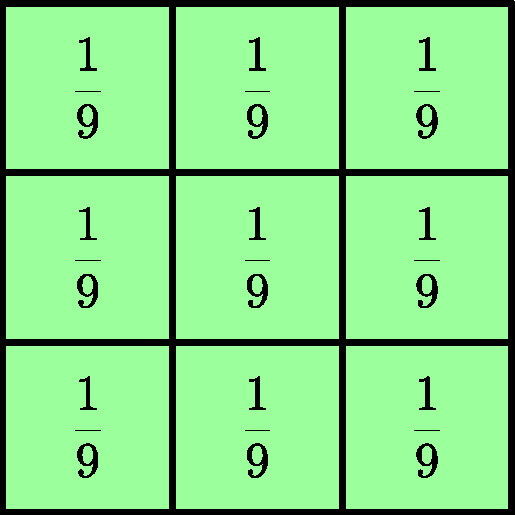
\includegraphics[height=2cm]{figs/maxmixed.pdf}
    %\caption{Maximally mixed state $\frac{1}{3}\id$}%
    }\hspace{8pt}%
    \subfigure[][]{%
    \label{fig:zero}%
    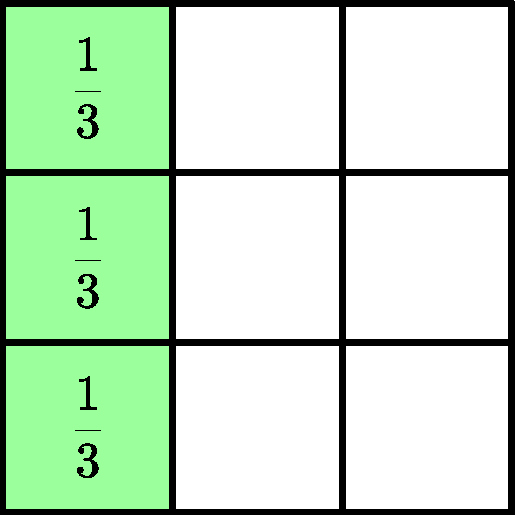
\includegraphics[height=2cm]{figs/zerostate.pdf}
    %\caption{Zero state $\ketbra{0}{0}$}%
    }\\
    \subfigure[][]{%
    \label{fig:bound}%
    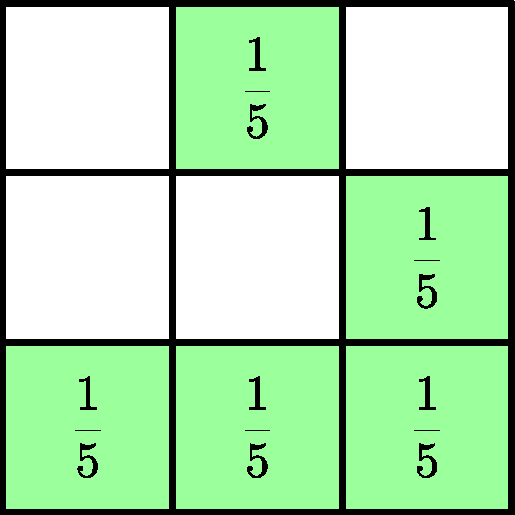
\includegraphics[height=2cm]{figs/boundstate.pdf}
    %\caption{Bound state}%
    }\hspace{8pt}%
    \subfigure[][]{%
    \label{fig:Strange}%
    \includegraphics[height=2cm]{figs/Strangestate.pdf}
    %\caption{Strange state $\ketbra{S}{S}$}%
    }
    \caption{\textbf{Qutrit Wigner distributions of varying magic.} 
    \subref{fig:maxmix} Maximally mixed state $\frac{1}{3}\id$; \subref{fig:zero} Stabilizer zero state $\ketbra{0}{0}$; \subref{fig:bound} A non-stabiliser Wigner-positive state; \subref{fig:Strange} Magic Strange state $\ket{{\rm{S}}} = \frac{1}{\sqrt{2}}(\ket{1} - \ket{2})$, coined in~\cite{cit:veitch2}.
    }%
    \label{fig:wstate_examples}
\end{figure}

Any quantum operation $\E$ can also admit a Wigner representation. If $\E$ maps some quantum system $A$ to a quantum system $B$, and $\J(\E)$ is its associated Choi state then we can define
\begin{equation}
W_{\E}(\y |\x) \coloneqq d_A^2 W_{\J(\E)}(\bar{\x} \oplus \y),
\end{equation}
where $\bar{x} =(x_1, -p_1, \dots , x_n, -p_n)$ can be viewed as the time-reversed version of $\x$ in the discrete phase space, where momenta are reflected while position coordinates remain unchanged.

\subsection{Magic theories for quantum computation}
\label{sec:mono}

A number of magic theories exist, with the central approach of viewing magic states as ``resource'' states with respect to a natural class of quantum operations that are considered free~\cite{Gour_2019}. One very natural class of free operations are those obtained from Clifford operations, measurements and the ability to discard quantum systems. However, there are also other noteworthy candidates~\cite{cit:ahmadi, cit:seddon, Wang_2019}.

In any theory of magic, a natural route to bounding the distillation rates obtainable is through the concept of a \emph{magic monotone}. A magic monotone is a real-valued function of any quantum state $\M(\rho)$ that is monotonically non-increasing under the free operations of the magic theory. More precisely $\M(\sigma) \le \M(\rho)$ whenever it is possible to convert $\rho$ into $\sigma$ using free operations (e.g. Clifford operations).

One of the most prominent magic monotones is the \emph{mana} of a state~\cite{cit:veitch2}, defined as
\begin{equation}
    \mana{\rho} \coloneqq \ln{(2\hspace{1pt}\sn{\rho}+1)},
\end{equation}
where the \emph{sum-negativity}~\cite{cit:veitch2} is the sum of the negative components in $\W{\rho}$,
\begin{equation}
    \sn{\rho} \coloneqq \sum\limits_{\bmx: \W[\bmx]{\rho} < 0} \abs{\W[\bmx]{\rho}}.
\end{equation}

Mana is an additive\footnote{It satisfies the condition $\mana{\rho_1 \otimes \rho_2} = \mana{\rho_1} + \mana{\rho_2}$ which is practical in distillation settings.} magic monotone, so it provides an analytical, necessary condition for many-copy magic state interconvertibility.

A range of monotones have been developed in the literature~\cite{cit:howard, Wang_2020, Seddon_2021} and each provides a means to upper bound distillation rates within a particular theory of magic. In this work we shall develop bounds that apply to essentially any reasonable magic theory. The central idea is to apply majorization theory to the quasi-probability distributions of magic states. In the next section, we explain how these majorization constraints relate to the free operations allowed in a theory of magic.


%%%%%%%%%%%%%%%%%%%%%%%%%%%%%%%%%%%%%%%%

\subsection{Stochastic structure of magic protocols}
\label{sec:struc}

Within the Wigner representation, all negatively represented states are magic states, although in general the converse is not true~\cite{cit:campbell}. However, it is known that all positively represented states used in Clifford circuits admit an efficient classical description, so it is natural to focus on the negatively represented magic states. The free states in any magic theory must therefore lie in the set
\begin{equation}
    \Fmax \coloneqq \{ \rho: \W[\bmx]{\rho} \geq 0 \text{ for all } \bmx \in \cal{P}_d\}.
\end{equation}
Our focus is on states with negativity, so the particular choice of free states is not critical for our analysis. The remaining component that defines any magic theory is the set of allowed (free) quantum operations, i.e. the ones that are considered free. The assumption we require on free operations is simply that they send any free state to another free state, meaning that a resource state cannot be created freely, a common assumption among all magic theories.

We can view the Wigner representation $W_{\E}( \y | \x)$ of a quantum channel $\E$ as a transition matrix mapping points $\x \rightarrow \y$, which is consistent with the representation of quantum states, as
\begin{equation}
	W_{\E(\rho)} (\y) = \sum_{\x \in \P_d} W_{\E}( \y | \x) W_\rho(\x),
\end{equation}
for any $\E$ and $\rho$. Now if $\E$ sends all positively represented quantum state to other positively represented quantum states then it can be shown~\cite{Wang_2019} that $W_{\E}(\y |\x)$ must form a stochastic matrix. In particular, all Clifford operations correspond to stochastic matrices in this Wigner representation. However, it is important to note that not all stochastic maps on the phase space correspond to valid quantum operations. In particular, the stochastic maps must respect the symplectic structure of the phase space, which is an additional non-trivial constraint.

In what follows we shall therefore assume that we have a magic theory $\R = (\F, \O)$ in which the free states $\F$ form a closed set with each state represented by a non-negative Wigner function, while the free operations $\O$ are represented by stochastic maps acting on the discrete phase space.


\section{Magic distillation bounds from majorization theory}
\label{sec:frag}

We wish to consider how physical constraints that may be hardware specific, affect magic distillation rates. These are not a priori encoded in the formulation of the magic theory, and constitute additional physical conditions on top of the underlying resource-theoretic accounting. For example, there may be non-trivial thermal noise in the physical set-up or the accessible operations, there might be strong bias in the noise present, or we might be limited in how easily certain gates can be realised.~\cite{Aliferis_2008, Stephens_2013, Li_2015, Babbush_2018, Tuckett_2019, Guillaud_2019, Fowler_2019}. \nick{repeats intro}

Our formulation will not consider model-specific limitations, but will still inject broad physical constraints. We proceed by considering fixed-point, or ``equilibrium'', restrictions on the actual operations that are accessible to us. While such restrictions could be viewed as the existence of some non-trivial thermodynamic constraint, they could equally be viewed as encoding a high noise-bias or difficulty in realising a particular quantum gate. We can therefore define the following sub-theory of any magic theory $\R$.
\begin{definition}[\textbf{$\boldsymbol\sigma$--fragment}]\label{def:sigmafrag}
   Given a theory of magic $\R = (\F, \O)$, the \emph{$\sigma$--fragment of $\R$} is the sub-theory $\R_\sigma = (\F, \O_\sigma)$, in which the free operations are 
   \begin{equation}
        \O_\sigma \coloneqq \{ \E \in \O: \E(\sigma) = \sigma \},
    \end{equation}
namely those operations that leave the state $\sigma \in \F$ invariant.
\end{definition}
This notion provides a simple way to break up any theory into smaller, more manageable parts that are destinguished by additional physical constraints, illustrated in~\cref{fig:zoo}. Moreover, the union over all fragments returns the parent theory, so we are not discarding any information by breaking up the theory in this way. We make this statement precise as follows.
\begin{theorem}\label{thm:frag}
    Let $\R = (\F, \O)$ be a theory of magic.
Then a transformation $\rho \longrightarrow \tau$ is possible in $\R$ if and only if the transformation $\rho \longrightarrow \tau$ is possible in at least one $\sigma$--fragment of $\R$.
\end{theorem}
\begin{proof}
	The proof is straightforward.
   Suppose the interconversion is possible in a $\sigma$--fragment via some $\E \in \O_\sigma$. But since $\O_\sigma \subseteq \O$ it is also possible in $\R$. Conversely, suppose the transformation is possible in $\R$ via some $\E$ in $\O$. The free states $\F$ are a closed, bounded set and moreover the image of $\F$ under the map $\E$ is in $\F$. By the Brouwer Fixed-Point theorem~\cite{cit:brouwer} this mapping must therefore have a fixed point $\sigma \in \F$. Therefore $\E \in \O_\sigma$ and so the interconversion is possible in this fragment.
\end{proof}

\begin{figure}[t]
    \centering
        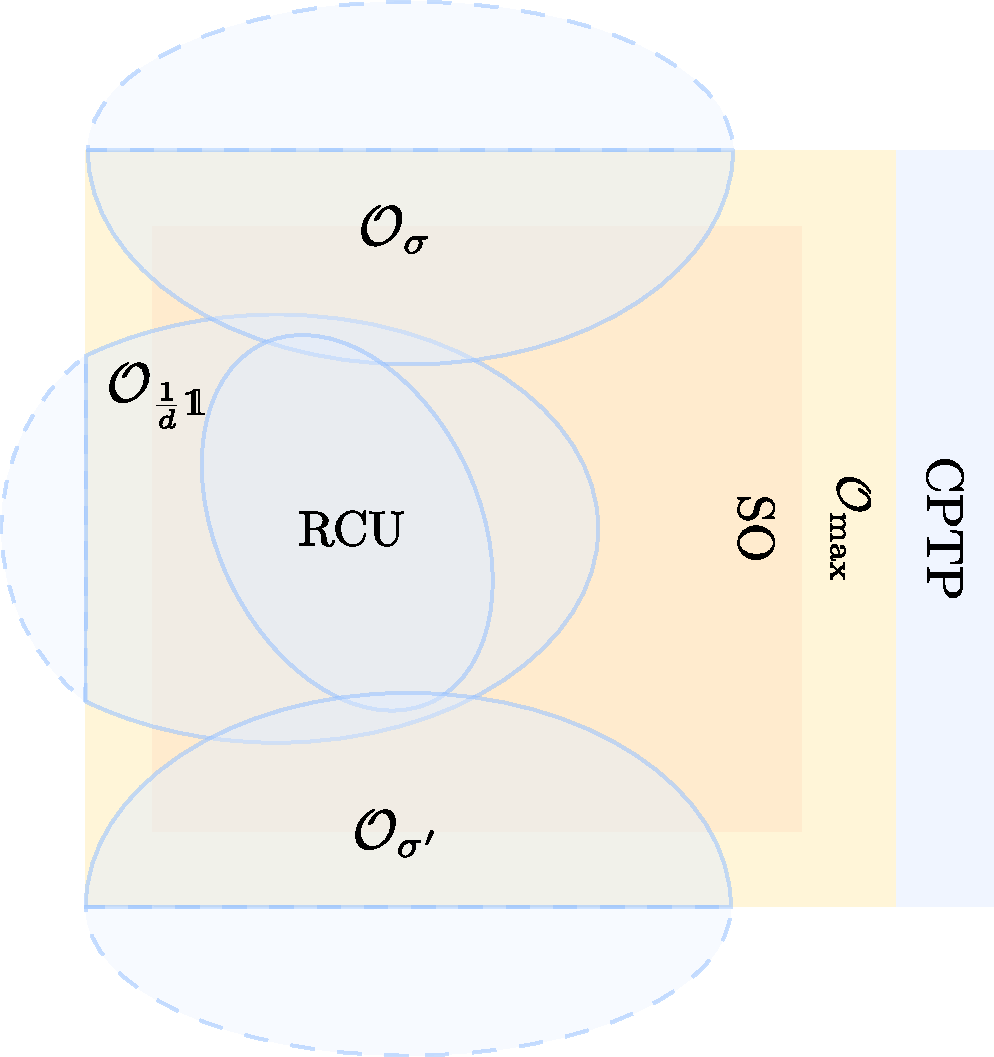
\includegraphics[scale=0.3
        ]{figs/operations.pdf}
    \caption{\textbf{Decomposition of a magic theory $\R$ into $\sigma$--fragments.} 
	Examples of magic theories ($\so$: Stabilizer operations, $\Omax$: Completely positive-Wigner-preserving operations, $\rcu$: Random Clifford Unitaries -- subclass of $\so$) are labelled, with other established magic theories also contained within the yellow regions.
    We introduce $\sigma$--fragments $\O_\sigma$ defined for all free states $\sigma$ that cover $\Omax$. 
    Each $\O_\sigma$ is extensible to a set of stochastic maps outside the $\cptp$ operations.
    Within each $\sigma$--fragment, relative majorisation can be used allowing for a tractable approach towards the study of magic state interconversions.
    }
    \label{fig:zoo}
\end{figure}

It is now possible to consider magic distillation rates within $\sigma$--fragments and then see how the bounds on the distillation rates depend on the choice of the fragment we work within. Therefore, this route can potentially shed light on how the physics of a protocol constrain distillation rates above and beyond global constraints from the parent resource theory. For example, how does temperature affect distillation bounds? Do isotropic maps have better bounds, or does bias towards some pure stabilizer state provide more freedom?
\nick{re-write based on new relative majorisation approach}

By introducing this additional structure to a magic theory, we allow for deeper analysis than would be possible at the level of the full parent theory. In particular, the interconversion structure in each fragment can be analysed using tools from single-shot thermodynamics and majorization theory as we discuss in the next section.

\subsection{Quantifying disorder without entropies}
\label{sec:major}

We can now show that each magic fragment admits constraints that do not take the form of state monotones. 

The question is now whether the sub-theories can be analysed to provide additional insights into magic distillation protocols. An answer can be provided by working in the Wigner representation of a given $\sigma$--fragment. The problem of magic state distillation then becomes that of processing negativity under stochastic maps $W_{\E}( \y |\x)$ that leave a particular quasi-distribution $W_\sigma(\x)$ invariant. However, $\sigma \in \F$ is positively represented, so the sub-theory has an invariant classical probability distribution as a fixed point. This structure allows us to make use of a range of classical tools, and in particular majorization theory.

Majorisation~\cite{cit:marshall} is a collection of powerful tools that has recently found many applications in quantum information theory~\cite{Nielsen_1999, cit:cwiklinski, cit:lostaglio2, cit:gour, cit:gour2, Horodecki_2003, Vallejos_2021}.
It describes the disorder of distributions that undergo stochastic transformations. In its simplest form it defines a pre-order on probability distributions. Given two distributions $\p= (p_1, \dots, p_n)$ and $\q = (q_1, \dots, q_n)$ over $n$ outcomes, we say that $\p$ majorises $\q$, denoted $\p \succ \q$, if there exists a bistochastic map $A = (A_{ij})$ such that $A\p = \q$, where bistochastic means that $A_{ij} \geq 0$ and $\sum_i A_{ij} = \sum_j A_{ij} = 1$. A well-known result~\cite{cit:marshall} tells us that the condition $ \p \succ \q$ over probability distributions is equivalent to $n-1$ inequalities, which can be checked efficiently.

There is a natural generalisation, which is called $\bmd$--majorization~\cite{Veinott_1971}, or in the context of thermodynamics, thermo-majorization \ddd{[cite]}. For a fixed probability distribution $\r = (r_1, \dots, r_n)$ with positive components, we define majorization relative to $\r$ as $\p \succ_{\r} \q$, if and only if there exists a stochastic map $A$ such that $A\r = \r$ and $A \p = \q$. In order words, the relative majorization pre-order coincides with the image of $\p$ under stochastic maps that have $\r$ as a fixed point. It is readily checked that the original majorization condition between probability distributions corresponds to the case $\r = (1/n, \dots, 1/n)$. The pre-order that results from relative majorization is also easily checked and again corresponds to checking a small number of inequalities.

We can further generalise this to \emph{relative majorization}\ddd{[cite]}, defined as an ordering between pairs of vectors so that 
\begin{equation}
	(\p,\r) \succ (\q, \r')
\end{equation}
iff there is a stochastic map $A$ such that $A\r = \r'$ and $A\p = \q$. We retrieve $\bmd$--majorization when $\r = \r'$.

It turns out that relative majorization is equally applicable to \emph{quasi-probability} distributions, and therefore can be applied to the Wigner representation of magic across fragments. We go into more detail on this in the next section.

\subsection{Quasi-probability majorization and non-monotonic Lorenz curves}
\label{sec:lc}

We wish to apply majorization to describing magic in different fragments at the level of the associated Wigner distributions. However, these are in general quasi-probability distributions and so it is important to detail how majorization is computed for these cases and what differences quasi-distributions bring over genuine probability distributions.

Central to the analysis is the notion of a Lorenz curve of a vector $\w \in \mathbb{R}^n$ relative to some other vector $\r \in \mathbb{R}^n$. Given a vector $\w$ we define $\w^\downarrow$ to be the re-arrangement of the components of $\w$ into decreasing order. Now, given two $n$--component vectors $\w$ and $\r$ we define the \emph{Lorenz curve} of $\w$ relative to $\r$, denoted $L_{\w|\r}(x)$, as the piece-wise linear function that passes through $(0,0)$ and the $n$ points
\begin{equation}
\label{eq:lc}
        (x_k,L_{\w|\r}(x_k)) =\left( \frac{1}{R}\sum_{i=1}^k r_{\pi(i)}, \sum_{i=1}^k w_{\pi(i)} \right),
\end{equation}
where $R:= \sum_{i=1}^n r_i$, and $\pi$ is the permutation on $n$ objects that sends $\widetilde{\w}$ to $\widetilde{\w}^{\downarrow}$, where $\widetilde{w}_i := w_i/r_i$ is the vector of component-wise ratios of $\w$ and $\r$. The form of this requires that $\r$ has no zero components, which we shall assume without loss of generality as in any physical situation the rank of a quantum state is not an operationally meaningful quantity.
We also observe that the curve contains non-differentiable points, called \emph{elbows} at locations where $\widetilde{\bmw}$ changes value.

If $\w$ and $\r$ are both probability distributions then the Lorenz curve is defined on the interval $[0,1]$, and rises monotonically until it reaches the value $1$ at $x=1$. The value $L_{\w|\r}(x) = 1$ is a global maximum, attained at the end-point $x=1$. Moreover, if $\w, \w', \r, \r'$ are all valid probability distributions with neither of $\r,\r'$ having negative components then it has been shownin~\cite{ruch_mixing_1978} that
\begin{equation}
(\w, \r) \succ (\w', \r') \mbox{ if and only if } L_{\w |\r}(x) \ge L_{\w' |\r'}(x).
\end{equation}
This provides a simple way of computing whether relative majorization holds between pairs of probability distributions.

However, if $\w$ is a \emph{quasi-probability} distribution with negative values, and $\r$ a regular probability distribution things are different. Now the Lorenz curve is no longer monotone increasing, but is a concave function that breaks through the $L_{\w|\r}(x) = 1$ barrier at an interior point and attains some non-trivial maximum $L_\star$ above the value $1$, before decreasing monotonically to $L_{\w|\r}(x)= 1$ at the end-point $x=1$. See Figure \ref{fig:lcs} for examples of non-monotonic Lorenz curves for quasi-distributions. Within quantum theory, the breaking of this barrier is associated with the degree of non-classicality. Since majorization provides a measure of order/disorder this is consistent with the intuition that negativity, for example within the context of entanglement theory or quantum computing, can provide a greater form of order than is possible within classical theory.

\begin{figure}
    \centering
    \includegraphics[height=4.5cm]{figs/lc_Strange.pdf}
    \caption{\textbf{A `heretical' family of Lorenz curves.} Traditionally, Lorenz curves for distributions are monotone increasing cumulant functions that reach a maximum value of $1$. In contrast, Lorenz curves for magic states break through the value of $L(x)=1$ due to the presence of negativity in the associated quasi-probability distributions. The above family of curves correspond to multiple copies of noisy Strange states $\rho_{\rm{S}}(\epsilon)^{\otimes n}$ (\cref{eq:noisysn}) for $n=1,2,3,4$ within a particular stabilizer fragment. Solid lines represent pure Strange states, while dashed lines represent noisy Strange states with depolarising noise ($\epsilon = 0.1$).
    }
    \label{fig:lcs}
\end{figure}

However, relative majorization is usually considered for probability distributions, and so we must verify that the same Lorenz curve conditions apply to quasi-probability distributions. This can be done from first principles, but a simpler way is see that this holds is to reduce to the problem of genuine distributions by first `masking' the negativity in the quasi-probability distribution $\w$ using the reference distribution $\r$ and then applying the conditions for relative majorization. 
 
More precisely, if the components of $\r$ are never zero, then there always exists an $\epsilon >0$ such that $\w_\epsilon := \epsilon \w + (1-\epsilon) \r$ is a genuine probability distribution. We can see that $(\w , \r) \succ (\w', \r')$ if and only if $(\w_\epsilon , \r) \succ (\w_\epsilon', \r')$, where we choose $\epsilon$ so that both $\w_\epsilon$ and $\w_\epsilon'$ are probability distributions. This equivalence holds because there exists a stochastic map $A$ such that $A \w = \w'$ and $A \r = \r'$ if and only if 
\begin{equation}
A[\epsilon \w + (1-\epsilon) \r] = \epsilon \w' + (1-\epsilon) \r'\mbox{ and } A\r = \r'.
\end{equation}
As mentioned, relative majorization between pairs of distributions occurs if and only if the associated Lorenz curves never cross. Therefore we can express this condition in terms of the Lorenz curves of the quasi-probability distributions $\w$ and $\w'$ relative to $\r$ and $\r'$ respectively.

As shown in Appendix \ref{lemma:Lorenz_linearity}, the Lorenz curve for any quasi-probability distribution obeys the following linearity condition
\begin{equation}
L_{a \w + b \r | \r} (x) = a L_{\w|\r} (x) + bx,
\end{equation}
for all $a >0$ and any $b \in \mathbb{R}$. We now have that
\begin{equation}
(\w, \r) \succ (\w', \r') \mbox{ if and only if } (\w_\epsilon , \r) \succ (\w_\epsilon', \r'),
\end{equation}
and also $(\w_\epsilon , \r) \succ (\w_\epsilon', \r')$ if and only if $L_{\w_\epsilon |\r} (x) \ge L_{\w'_\epsilon |\r'} (x)$ for all $x$. However, using the above linearity property of the Lorenz curves we have that
\begin{align}
L_{\w_\epsilon |\r} (x) &\ge L_{\w'_\epsilon |\r'} (x) \nonumber \\ 
&\mbox{ if and only if }& \nonumber \\
\epsilon L_{\w |\r} (x) + (1-\epsilon) x &\ge \epsilon L_{\w' |\r'} (x) + (1-\epsilon) x.
\end{align}
The $(1-\epsilon)$ terms cancel on both sides and we get the required relative majorization conditions for the quasi-distributions in terms of their Lorenz curves.

We therefore have that $(\w, \r) \succ (\w', \r')$ if and only if $L_{\w | \r} (x) \ge L_{\w' | \r'}(x)$ for all $x \in [0,1]$ equally applies for the case of $\w,\w'$ being quasi-distributions. 

In the next section we discuss the application of majorization to Wigner representations of magic, where the quasi-distribution $W_\rho(x)$ of a magic state can be analysed relative to any Wigner positive free state $W_\sigma(x)$. To our knowledge, the application of majorization to quasi-distributions in  physics has not been considered previously. The caveat here is that relative majorization ranges over stochastic maps that obey a transformation ($A\r = \r'$), while in the case of the Wigner representation there is a stronger restriction that the symplectic structure of the phase space is respected. Therefore, any majorization constraint can provide necessary, but not sufficient conditions on magic state interconversions. This observation raises a question that to our knowledge has not been previously considered in the classical statistical mechanics literature: what are the conditions for symplectic majorization of classical statistical mechanics? We shall \nick{return} to this question later on when we discuss how our approach could be used to construct concrete lower-bounds on distillation rates in~\cref{sec:lower_bounds}.

\subsection{Majorisation of negative Wigner distributions within $\sigma$--fragments}
\label{sec:major_frag}

Having described how majorization relative to a fiducial distribution can be computed, we now turn to its application within a particular fragment of a magic theory $\R= (\F, \O)$.

If we consider some $\sigma \in \F$, and its corresponding fragment $\R_\sigma$, then we are typically interested in the ability to transform many copies of some magic state $\rho$ into more pure forms of magic. The state $\rho$ is assumed to have negativity in the Wigner representation, so $W_\rho(\x) < 0$ for some regions of $\x \in \P_d$. We again note that we restrict to odd-dimensional quantum systems, for simplicity. In contrast, the state $\sigma$ will have a Wigner distribution $W_\sigma(\x)$ that forms a genuine probability distribution. On the technical assumption that $\sigma$ is full rank, we also have that $W_\sigma(\x) > 0$ for all $\x \in \P_d$. Any non-full rank states $\sigma$ can be handled as a limiting case in which we inject an infinitesimal fraction of depolarising noise $\epsilon (\id/d)$.

As discussed already, the free operations within the magic theory $\R$ are represented by stochastic maps, and within $\R_\sigma$ by stochastic maps that leave $W_\sigma(\x)$ invariant. Therefore, a necessary condition for magic state transformations $\rho_1 \rightarrow \rho_2$ within $\R_\sigma$ will be that 
\begin{equation}
W_{\rho_1} \succ_{W_{\sigma}} W_{\rho_2},
\end{equation}
or put another way, relative to $W_\sigma$ the quasi-distribution $W_{\rho_1}$ is more ordered than the quasi-distribution $W_{\rho_2}$. 

This in turn can be expressed in terms of Lorenz curves. To simplify notation we denote by $L_{\rho | \sigma}(x)$ the Lorenz curve $L_{W_{\rho} | W_{\sigma}} (x)$. We therefore have that
\begin{equation}
\rho_1 \rightarrow \rho_2 \mbox{ within }\R_\sigma \mbox{ implies } L_{\rho_1 |\sigma} (x) \ge L_{\rho_2 |\sigma} (x),
\end{equation}
for all $x \in [0,1]$. Therefore, the magic state Lorenz curve condition can be used to impose upper bounds on magic distillation rates. Note, however, that unlike any monotone, this is not a single numerical constraint, but a \emph{family} of constraints. Indeed, for $n$ copies of a $d$--dimensional system the number of terms in $W_{\rho}$ is $d^{2n}$, so the Lorenz curve condition corresponds to \emph{exponentially} many constraints, of which there are as many independent constraints as there are elbows in the Lorenz curve of the output state, which is proved in~\cref{thm:elbows} in~\cref{app:frag}.
In principle, any one location $x$ provides a valid constraint leading to some upper distillation bound and optimising over the location provides the strictest bound.

\subsection{Basic monotones for magic states in a particular fragment}
\label{sec:monotones_frag}

In this section we give some generic aspects of Lorenz curves for magic states. In particular these allow us to interpret previous magic monotones in a new light. The f,irst result provides an extremely simple way to see that the sum-negativity of a magic state is a monotone.

\begin{lemma} Relative majorization in any fragment implies the monotonicity of sum-negativity. 
\end{lemma}
\begin{proof}
	The sum-negativity of a magic state $\rho$ can be written as $sn(\rho) := \frac{1}{2} (\sum_{\x} |W_\rho(\x) | - 1)$.
We make use of a variant form of relative majorization, (see~\cref{prop:rmajor} in~\cref{app:major}), stating that $\p \succ_{\r} \q$ if and only if
	\begin{equation}
\sum_k | p_k - r_k t | \geq \sum_k | q_k - r_k t |,
\end{equation}
for all $t\in \mathbb{R}$. Choosing $t=0$ we get the single condition that $\sum_k |p_k| \ge |\sum_k |q_k|$, independent of the choice of $\r$. Applying this to the Wigner quasi-distributions of two quantum states immediately gives the result.
\end{proof}
As a corollary, this result applies to mana too, since mana is an increasing function of sum-negativity.

If we have a magic state $\rho$ that has negativity in its Wigner representation, then as discussed, its Lorenz curve over-shoots $1$ and reaches a non-trivial maximum $L_\star$ that depends on the particular state. There is an exact relation between the peak and sum-negativity or mana, which is provided by the following result. 
\begin{lemma}\label{lem:lcmax}
	Given a magic state $\rho$, the maximum $L_\star$ of its Lorenz curve $\lc{\rho}{\sigma}(x)$ is independent of the $\sigma$--fragment and equal to $1+\sn{\rho}$. Moreover, the majorization constraint is stronger than mana in every fragment.
\end{lemma}
The proof of this is given in Appendix \ref{lem:lcmax}. Using the Lorenz curve perspective, it is simple to construct other monotones. For example, within a given fragment, the area above $L=1$ is another magic monotone.
\begin{lemma} Let $\A_\sigma(\rho)$ be the area of the region $\{(x,y) : (x, L_{\rho | \sigma}(x)) \ge 1\}$. Then $\A_\sigma(\rho)$ is a magic monotone for $\R_\sigma$.
\end{lemma}
\begin{proof}
Consider the transformation $\rho_1 \rightarrow \rho_2$ within $\R_\sigma$. We have that $L_{\rho_1|\sigma}(x)$ is never below the curve $L_{\rho_2|\sigma}(x)$, and therefore the region above $L=1$ for $\rho_2$ is a subset of the corresponding region for $\rho_1$. Thus, $\A_\sigma(\rho_1) \geq \A_\sigma(\rho_2)$, so $\A_\sigma$ is a magic monotone in $\R_\sigma$.
\end{proof}
In contrast to mana, the area monotone is \emph{specific to the fragment}, and its value will vary as we change $\sigma$. Therefore its monotonicity is also including the physics of the fragment and provides a means to analyse magic distillation only under free operations that leave $\sigma$ invariant.

We ultimately want to make statements about asymptotic distillation rates $R$,
\begin{equation}
\rho_1^{\otimes N} \longrightarrow \rho_2^{\otimes R N}
\end{equation}
where $\rho_2$ is a purer magic state than $\rho_1$ and $R$ is made as large as possible as $N$ tends to infinity. We shall next turn to this analysis, and exploit basic features of a magic state in order to obtain non-trivial distillation bounds.


\subsection{Magic bounds for unital protocols}
\label{sec:unital}

In this section, we apply majorization to magic state distillation within a simple fragment, namely the unital fragment. This encompasses distillation protocols where one is restricted to \emph{unital operations}, meaning that $\E(\I/d) = \I/d$ for all free $\E$. This is a particularly powerful set of operations, which for example include all Weyl-covariant channels~\cite{cit:gross3}. To make things concrete, we shall consider qutrit magic states ($d=3$) as the Wigner representation is simpler compared to qubits ($d=2$), while they admit non-trivial structure (e.g. Hamiltonians with two different energy gaps) and still are sufficiently simple to analyse in detail.

For our distillation protocols we need to choose a canonical pure magic state as a target. For this we shall choose the Strange state $|S\>$ given as
\begin{equation}
|S\> := \frac{1}{\sqrt{2}} (|1\> + |2\>),
\end{equation}
in the computational basis. This qutrit magic state is exceptionally symmetric and simple which benefits our analysis. Its distribution $W_S(\x)$ has a single negative value of $-1/3$ at $\x =(0,0)$ and the positive value $1/6$ at all other points. We can define the $\epsilon$--noisy Strange state as
\begin{equation}\label{eq:noisysn}
    \rho_{\rm{S}}(\epsilon)\coloneqq (1 - \epsilon) \ket{\rm{S}}\bra{\rm{S}} + \epsilon \frac{1}{3}\id,
\end{equation}
where $\epsilon$ is the depolarization noise parameter. Moreover, utilising the symmetries of the Strange state allow for any magic state $\rho$ to be processed via Clifford operations~\cite{cit:prakash,cit:prakash2} and put into this canonical form for some $\epsilon \ge 0$.

The Wigner distribution of the single-copy, $\epsilon$--noisy Strange state  is given by
\begin{equation}
	\W[\bmx]{\rho_{\rm{S}}(\epsilon)} = (1-\epsilon)\W[\bmx]{\ketbra{\rm{S}}} + \epsilon\W[\bmx]{\frac{1}{3}\id}.
\end{equation}
Since the Wigner distribution $W_{\I/3}(x)$ is the uniform probability distribution over the phase space, we get that $W_{\rho_S(\epsilon) } (\x)$ has a single negative component
\begin{equation}
	- v(\epsilon) \coloneqq - \left( \frac{1}{3} -\frac{4}{9}\epsilon \right)
\end{equation} 
located at the origin $\bmx = \bmo$ and positive components
\begin{equation}
	u(\epsilon) \coloneqq \frac{1}{6} -\frac{1}{18}\epsilon
\end{equation}
at the 8 phase space points $\x \ne (0,0)$. We assume that $\epsilon < 3/4$ to ensure the presence of negativity in the Wigner distribution. 

We now consider the task of purifying $n$ copies of a noisy Strange state $\rho_{\rm{S}}(\epsilon)^{\otimes n}$ as given in~\cref{eq:noisysn} into a smaller number of copies $n'$ of a less noisy Strange state $\rho_{\rm{S}}(\epsilon')^{\otimes n'}$, with $\epsilon' < \epsilon$ and $n' \leq n$. Since we work in the unital fragment, the maximally mixed state is free and we choose to tensor in $n'-n$ auxiliary copies of it to the output, highlighting that we are working in the unital fragment. This affects neither the distillation process nor our analysis, since the Lorenz curves remain unaffected. More generally, it is easy to see that
\begin{equation}
	L_{\rho |\sigma} (x) = L_{\rho \otimes \sigma |\sigma \otimes \sigma}(x),
\end{equation}
for any full-rank $\sigma \in \F$. Therefore, we consider the transformation
\begin{equation}\label{eq:sudist}
	\rho_{\rm{S}}(\epsilon)^{\otimes n} \longrightarrow \rho_{\rm{S}}(\epsilon')^{\otimes n'} \otimes \left( \frac{1}{3}\id \right)^{\otimes (n-n')},
\end{equation}
and compare the Lorenz curves for the input and output states to bound $R(\epsilon, \epsilon') \coloneqq n'/n$, the rate of this interconversion within the fragment.

The Wigner distribution of $n$ copies of the state is obtained by the $n$-fold product of the single copy distribution, and the Lorenz curve $L_{\rho|\sigma}(x)$ for $\rho = \rho_S(\epsilon)^{\otimes n}$ and $\sigma = (\I/3)^{\otimes n}$ is readily computed for any $n$ and $\epsilon$, and the full details are provided in~\cref{app:lcsu_technical}.
We highlight that the non-trivial element that arises for quasi-distributions is that the product of negative components can generate a positive $n$-fold component, so the ordering of the components of $W_{\rho |\sigma}(x)$ depends on whether $-v(\epsilon)$ appears to an even or odd power in the expression of~\cref{eq:wigu}.

The component values $w_i$ and associated multiplicities ($m_i$) in the $n$--copy case are 
\begin{align}
	m_i &= 8^{i}\binom{n}{i}, \\
	w_i &= u^{i}(-v)^{n-i}, \label{eq:wigu}
\end{align}
where index $i$ runs through $0, \dots, n$, and we assume for simplicity of exposition that $n$ is even and the noise level is not high, $\epsilon \leq 3/7$, so that $v \geq u$.
The details of this scenario, along with the other possible cases that occur depending on the noise level and the parity of the number of copies, are provided in~\cref{app:lcsu_technical}.

The Lorenz curve $L_{\rho|\sigma}(x)$ rises monotonically and reaches a maximum value
\begin{align}\label{eq:lcsu_max}
	L_\star &\coloneqq L_{\rho |\sigma} (x_\star) = \sum_{i = 0}^{n/2} m_{2i} w_{2i} \nonumber\\
	&= \frac{1}{2} + \frac{1}{2}\left(\frac{15 - 8\epsilon}{9}\right)^n > 1,
\end{align}
which occurs at $x=x_\star$ given by
\begin{equation}
	x_\star = \frac{1}{2} + \frac{1}{2}\left(\frac{7}{9}\right)^n.
\end{equation}

It is possible to derive distillation bounds from any location of the Lorenz curve, including the region around the peak, by imposing the constraint that the Lorenz curve of the input state never dips below the curve of the output.
However, it turns out that a simple and sufficiently non-trivial constraint can be obtained by considering the first elbow of the Lorenz curves. 
The largest Wigner component occurs for $i=0$ and is unique, so the first elbow coordinates for $\rho_S(\epsilon)^{\otimes n}$ are given by $(1/9^n, v(\epsilon)^n)$, while for $\rho_S(\epsilon')^{\otimes n'}$ by $(1/9^{n'}, v(\epsilon')^{n'})$.

The first elbow constraint involves a simple interpolation, done in~\cref{app:elb_constraints}, in order to find the coordinates of both Lorenz curve points at the location where the first elbow occurs. 
Comparing these two points leads to the bound
\begin{equation}
	R(\epsilon, \epsilon') \leq \frac{\ln{(3-4\epsilon)}}{\ln{(3-4\epsilon')}}.
\end{equation}
For the limiting case of distilling pure magic states ($\epsilon'=0$), we obtain an upper bound in the unital fragment given by
\begin{equation}
	R \leq 1 + \frac{\ln (1 - \frac{4}{3} \epsilon)}{\ln 3}.
\end{equation}

Similar upper bounds on distillation rates for qudits of odd prime dimension include the mana bound~\cite{cit:veitch} and the max--thauma bound~\cite{Wang_2020} which is defined via a semi-definite program, but possesses properties that allow for an easy comparison with our bound.
The mana bound can be directly calculated as
\begin{equation}
	R \leq \frac{\mana{\rho_{\rm{S}}(\epsilon)}}{\mana{\rho_{\rm{S}}(0)}} = 1 + \frac{\ln \left(1 - \frac{8}{15}\epsilon \right)}{\ln \frac{5}{3}}.
\end{equation}
Using the max--thauma properties of super-additivity and vanishing at free states, we obtain
\begin{align}
	&\theta_{\rm{max}}(\rho_{\rm{S}}(\epsilon)) \geq (1-\epsilon) \theta_{\rm{max}}(\ketbra{\rm{S}}) + \epsilon \theta_{\rm{max}}\left(\frac{1}{3}\id \right) = \nonumber\\
	&(1-\epsilon) \theta_{\rm{max}}(\rho_{\rm{S}}(0)),
\end{align}
so that for a deterministic single-copy distillation process, an initial number of copies $n \geq \theta_{\rm{max}}(\tau) / \theta_{\rm{max}}(\rho) \geq 1-\epsilon$ is required.
Therefore, the max--thauma bound for the pure Strange state distillation process can get as tight as \nick{CALCULATING THAUMA EXACTLY AT THE MOMENT}
\begin{equation}
	R = \frac{1}{n} = \frac{\theta_{\rm{max}}(\rho_{\rm{S}}(\epsilon))}{\theta_{\rm{max}}(\rho_{\rm{S}}(0))} \leq 1-\epsilon.
\end{equation}

Both the mana and the max--thauma bounds are looser than the majorization bound we derived via the first elbow constraint as illustrated in~\cref{fig:distill_bounds}. 

In the next section we provide relative majorization bounds in arbitrary stabilizer fragments, and in particular we shall parameterize these bounds from a thermodynamic perspective. Specifically, we can interpret the stabilizer state $\sigma$, which defines the fragment, as a thermodynamic equilibrium state at some effective temperature and with some effective Hamiltonian.
\begin{figure}[t]
    \centering
    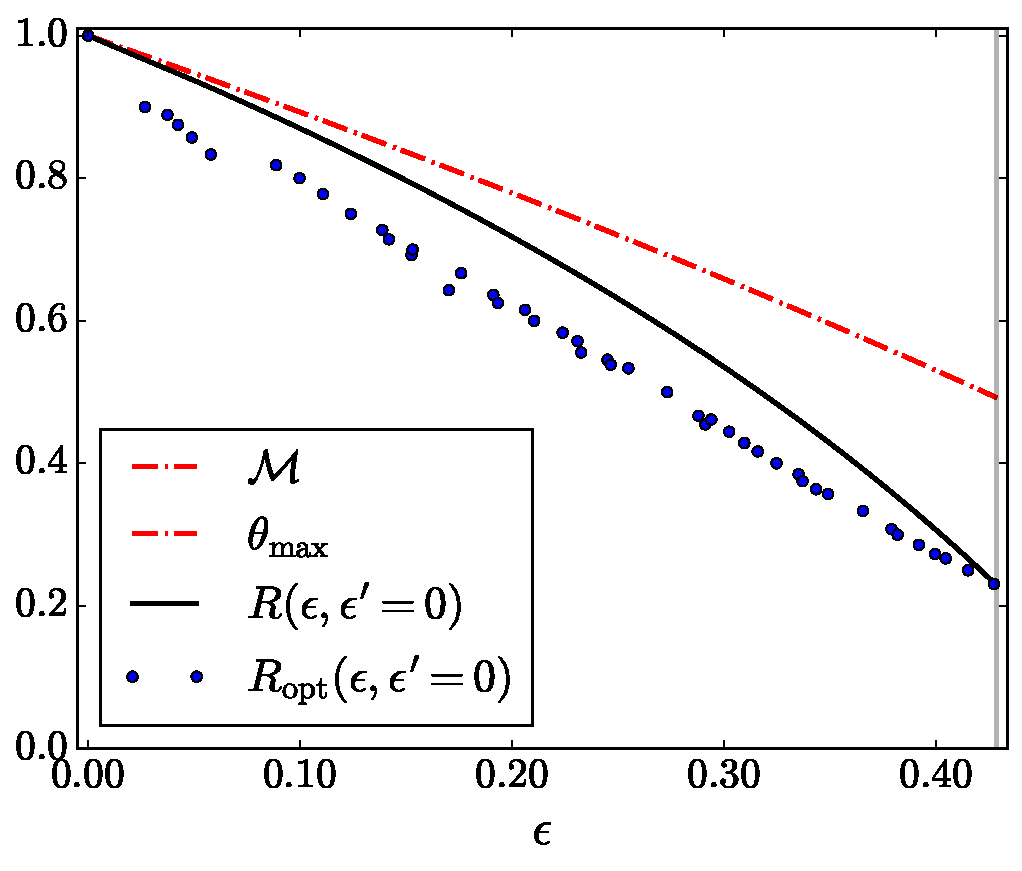
\includegraphics[scale=0.45]{figs/distill_bounds.pdf}
    \caption{\textbf{Distillation bounds in the unital fragment.} Distillation bounds obtained by majorisation, mana and the line $1-\epsilon$ (tightest bound of max--thauma) are plotted for $\epsilon' = 0$, up to noise level $\epsilon = 3/7$.
    Majorisation provides stricter rates than the global mana and max--thauma bounds.
    }
    \label{fig:distill_bounds}
\end{figure}

\section{Free energy dependent bounds for magic state distillation protocols}
\label{sec:stab}

We now consider a magic distillation protocol on multiple identical qudits in a noisy magic state $\rho(\epsilon)$, with noise parameter $\epsilon$, sending 
\begin{equation}
\rho(\epsilon)^{\otimes n} \longrightarrow \E(\rho(\epsilon)^{\otimes n}) =\rho(\epsilon')^{\otimes m}
\end{equation}
with $n \gg 1$, $\epsilon' <\epsilon$ and $\E$ denoting the quantum channel induced by the protocol. We can now provide distillation bounds that depend on energetic and entropic aspects of the protocol. We do this relative to a reference temperature that can be chosen freely. The key ideas is that the physical measures associated with this protocol are determined by how $\E$ would disturb this reference equilibrium state $\tau$ to some different state $\tau'$, if the protocol had been applied to this reference state instead of the $n$-copy magic state. 

More precisely, we assume each qudit has Hamiltonian $H$ and we choose some temperature $T = (k\beta)^{-1}$ where $k$ is Boltzmann's constant and $\beta$ the inverse temperature. The reference equilibrium state of the $n$ qudits is given by
\begin{equation}
\tau^{\otimes n} = \left ( \frac{e^{-\beta H}}{\Z} \right )  ^{\otimes n}.
\end{equation}
Since we are concerned with magic distillation we may assume that the reference state $\tau$ is not a magic state, and so has non-negative Wigner distribution, and we shall assume that it is a full-rank stabilizer state for the qudit. 

A given magic protocol on the $n$ qudits will correspond to a quantum channel $\E$. Our analysis associates to this protocol energy/entropy measures by considering how $\E$ transforms this reference equilibrium state. We first note that we can assume without loss of generality that $U_\pi\E(X) U_\pi^\dagger = \E(X)$ for any permutation $U_\pi$ of the $m$ output subsystems. The reason for this is that the protocol on the noisy magic state outputs the state $\rho(\epsilon')^{\otimes m}$, which is invariant under permutations, and so we can therefore always symmetrise by performing a group average over the permutation group for the output systems without changing the performance of the distillation protocol on $\rho(\epsilon)^{\otimes n}$. Thus, we can assume that $\E$ always outputs a symmetric state in general.

This means in particular that $\E(\tau^{\otimes n}) = \tau'$ is a symmetric state on $m$ subsystems, and so by the quantum de Finetti theorem \ddd{[cite]} we have that
\begin{equation}
\tau'  = \int d\mu(x) \sigma_x^{\otimes m},
\end{equation}
where $d\mu(x)$ is a probability measure over a set $\{\sigma_x\}$ of single qudit states.

To simplify our analysis we now make the following assumption. We assume that in the asymptotic/thermodynamic limit $n,m \rightarrow \infty$ that correlations generated in $\sigma$ are negligible. This implies that $d\mu(x)$ is peaked on a particular state $\sigma$, and so $\tau' = \sigma^{\otimes m}$. Physically, this is a natural scenario -- for example in traditional thermodynamics it states that the output system is well-described by intrinsic variables that are encoded in $\sigma$. Here this assumption allows us to associate a free energy per qudit for the output state, which would be more complex if correlations are present.

The case of correlations between output subsystems can also be considered, but would lead to a more complex analysis within our majorization analysis of Wigner distributions. In this direction we highlight recent work in majorization in which stochastic independence and correlations are analysed. In particular it has been shown that stochastic independence (no correlations) of independent distributions can be viewed as a resource in an extension of catalytic majorization, and leads to a single-shot operational interpretation of the Shannon entropy.

The action of the protocol on the reference states therefore transforms $\tau \rightarrow \sigma$. It turns out our distillation bounds depend on the free energy of the input and output states. For a state $\tau = e^{-\beta H}/\Z$ the associated free energy $F$ is given by
\begin{equation}
	F \coloneqq \tr[H \tau] - \beta^{-1}S(\tau) = -\beta^{-1}\log{\Z}.
\end{equation}
The output state $\sigma$ is generally a non-equilibrium state for the system. However, the distillation bound takes a particularly simple form if we associate a similar free energy value to the output state. We do this by considering the change in Hamiltonian $H \rightarrow H'$ such that equilibrium is restored at the reference temperature $T$. This implies that 
\begin{equation}
\sigma = \frac{e^{-\beta H'}}{\Z'},
\end{equation}
which has free energy $F' = -\beta^{-1} \log \Z'$. Therefore the action of $\E$ sending $\tau$ to $\sigma$ is viewed in terms of $\Delta H := H'-H$, which is the Hamiltonian change that would be needed to adiabatically restore equilibrium at temperature $T$. 

 Given this account of the physical ingredients of a distillation protocol we now state the following result for the case of qutrits.
\begin{theorem}\label{thm:free-energy}
	Consider a magic distillation protocol transforming noisy Strange state $\rho_S(\epsilon)^{\otimes n} \longrightarrow \E(\rho_S(\epsilon)^{\otimes n})=\rho_S(\epsilon')^{\otimes m}$ with $n, m \gg 1$.

Let each qutrit have a Hamiltonian $H$ with energies $E_0, E_1, E_2$, and define $E_{\rm max} = \max\{E_0, E_1, E_2\}$ and $E_s$ the eigenvalue of the eigenstate that overlaps the negative component of $\rho_S(\epsilon)$ in the Wigner representation. Let $T =(k\beta)^{-1}$ be any characteristic temperature for the physical system in the state $\tau^{\otimes n}= (e^{-\beta H}/\Z)^{\otimes n}$, with free energy $F$. Assume that for $n,m \gg 1$ the channel $\E$ generates negligible correlations on $\tau^{\otimes n}$, and so $\E(\tau^{\otimes n}) = \sigma^{\otimes m}$ for some state $\sigma$.

Define $\beta_\star = 1/kT_\star$ through the relation
\begin{equation}
	E_{\rm max} - E_s \eqqcolon kT_\star \ln 2,
\end{equation}
and define a threshold noise,
\begin{equation}
	\epsilon_{\star}(\beta) \coloneqq 
	\begin{cases}
		3 - \dfrac{18}{8-2^{\beta/\beta_\star}}, &\text{ for } \beta \leq \beta_\star \\
		0, &\text{ for } \beta > \beta_\star.
	\end{cases}
\end{equation}
Then the distillation rate $R = m/n$ of the magic protocol is bounded as:
\begin{equation}\label{eq:rate_bounds_proof}
	R \leq
	\begin{cases}
		\dfrac{\ln{\big( 1-\frac{4}{3}\epsilon \big)} + \beta (E_s - F)}{\ln{\big( 1-\frac{4}{3}\epsilon' \big)} + \beta (E'_s - F')},\ &\epsilon \leq \epsilon_\star, \epsilon' \leq \epsilon'_\star, \vspace{10pt}\\
		\dfrac{\ln{\big( 1-\frac{4}{3}\epsilon \big)} + \beta (E_s - F)}{\ln{\big( \frac{1}{2}-\frac{1}{6}\epsilon' \big)} + \beta (E'_{\rm{max}} - F')},\ &\epsilon \leq \epsilon_\star, \epsilon' > \epsilon'_\star, \vspace{10pt}\\
		\dfrac{\ln{\big( \frac{1}{2}-\frac{1}{6}\epsilon \big)} + \beta (E_{\rm{max}} - F)}{\ln{\big( 1-\frac{4}{3}\epsilon' \big)} + \beta (E'_s - F')},\ &\epsilon > \epsilon_\star, \epsilon' \leq \epsilon'_\star, \vspace{10pt}\\
		\dfrac{\ln{\big( \frac{1}{2}-\frac{1}{6}\epsilon \big)} + \beta (E_{\rm{max}} - F)}{\ln{\big( \frac{1}{2}-\frac{1}{6}\epsilon' \big)} + \beta (E'_{\rm{max}} - F')},\ &\epsilon > \epsilon_\star, \epsilon' > \epsilon'_\star.
	\end{cases}
\end{equation}
Where $F'$ is the free energy of the state $\sigma = e^{-\beta H'}/\Z'$ and other primed quantities are defined in the same way as the corresponding unprimed quantities. 
\end{theorem}

  For example, suppose that $H=H'$ then this implies the protocol would leave the equilibrium state unchanged and so corresponds to a Gibbs-preserving map \ddd{[cite Philippe]}. In the more general case $\Delta F := F' - F \ne 0$ and we have a free energy difference between the initial and final times, with respect to the relevant Hamiltonians. This is similar to the free energy differences that occur in fluctuation relations, where the final state of the system can be arbitrarily far from equilibrium, yet a free energy term for the final system still arises.
Firstly, the specific numerical factors in $\epsilon_\star$ are a result of our choice of magic state. 
Secondly, these bounds are derived based on analysis of only a part of the Lorenz curves and can be improved via a finer analysis. 
This is apparent by simple numerical calculations on the entirety of the curves.
Specifically, the existing bounds follow by considering the dominant terms in the rescaled Wigner distribution and do not, for example, take into account the Lorenz curve's peak structure. 


The above bounds mainly demonstrate how one can use relative majorization of quasi-distributions to incorporate additional information into distillation bounds. However to unpack the results more it is useful to consider the case in which $H=H'$, and look at $\epsilon' \rightarrow 0$. For this we obtain Figure \ref{contour-bounds} which gives a contour plot of $R$ as a function of inverse temperature $\beta$ and depolarising noise level $\epsilon$ for the initial noisy magic state.
\begin{figure}[t!]\label{contour-bounds}
    \centering
    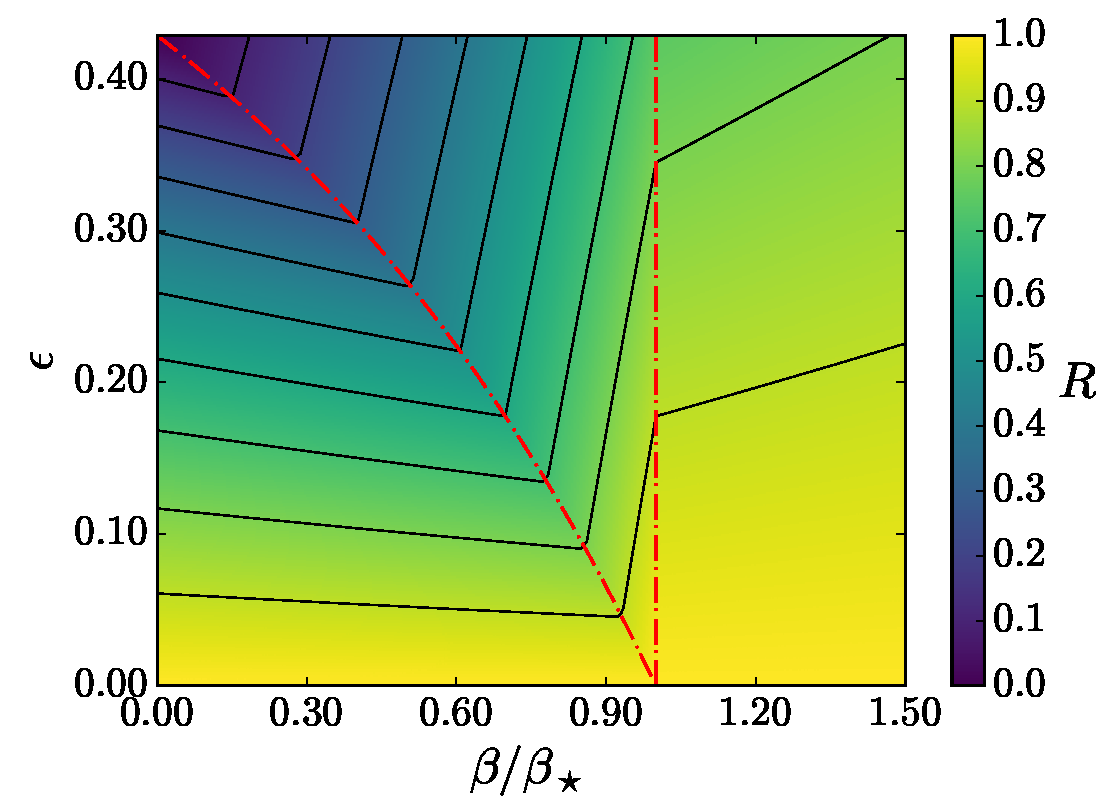
\includegraphics[scale=0.4]{figs/rate_scatter.pdf}
    \caption{\textbf{Temperature-dependent bounds for magic distillation.}
  Shown is a contour plot of  $R(\epsilon, \beta)$ where $\beta$ is an inverse temperature and $\epsilon$ is the depolarising noise of the magic state. The relevant data from the spectrum of the qutrit operator $H$ enters in via $\epsilon_\star(\beta)$ and $\beta_\star$.  The vertical dashed line is the `Landauer-like' temperature threshold $\beta_\star$ and the diagonal dashed curve corresponds to the noise threshold $\epsilon_\star (\beta)$ for $\beta \leq \beta_\star$. The $\beta =0 $ line corresponds to the regime in which the magic protocol gives a unital channel.
    }
    \label{fig:rate_contour}
\end{figure}
\begin{proof}
	We provide the full proof here, with some technical details pushed to~\cref{app:lcst_technical}.\\

Let $\displaystyle \sigma = e^{-\beta H} / \Z_\beta$ be a stabiliser state, where $\beta \geq 0$ and $H = E_0 \ketbra{\varphi_0} + E_1 \ketbra{\varphi_1} + E_2 \ketbra{\varphi_2}$ is an eigendecomposition of $H$.
The stabilizer state $\sigma$ can now be written as 
\begin{equation}
	\sigma = \frac{e^{-\beta E_0}}{\Z_\beta} \ketbra{\varphi_0} + \frac{e^{-\beta E_1}}{\Z_\beta} \ketbra{\varphi_1} + \frac{e^{-\beta E_2}}{\Z_\beta} \ketbra{\varphi_2},
\end{equation}
where $\{\ket{\varphi_k}\<\varphi_k|\}$ are pure, orthonormal stabiliser states, which can be represented in terms of generalized Paulis. To make our analysis simpler we perform a change of basis that does not affect the Wigner negativity of the problem. We let $C$ be the unitary transforming each $|\varphi_k\>\<\varphi_k|$ to $|k\>\<k|$. Since the Clifford group is the normalizer of the Heisenberg-Weyl group, $C$ is a Clifford unitary. Therefore, $C$ maps $\sigma$ to another stabilizer state that is diagonal in the computational basis, and we can assume without loss of generality that $\sigma$ is diagonal in $\{|0\>,|1\>, |2\>\}$. However, this choice means that the location of the negative Wigner component $-v(\epsilon)$ of the Strange state will be permuted on the discrete phase space. We denote by $E_s$ the eigenvalue of $H$ where the associated eigenvector has Wigner distribution overlapping the negative component of the magic state $C\rho_S(\epsilon)C^\dagger$.  This is unique, since the eigenstates form an orthonormal basis.

The Wigner distribution of state $\sigma$ is then given by
\begin{align}
	\W[\bmx]{\sigma} &= \sum\limits_{k=0}^2 \frac{e^{-\beta E_k}}{\Z_\beta}W_{\ketbra{k}}(x, p) \nonumber\\
	&= \sum\limits_{k=0}^2 \frac{e^{-\beta E_k}}{\Z_\beta} \delta_{x, k} = \frac{e^{-\beta E_x}}{3\Z_\beta},
\end{align}
where $x$ labels one of the three vertical lines in the phase space.
Since we have restricted to full-rank states, all Wigner components are strictly positive, and so the pre-order $\prec_{\sigma}$ is well-defined. States that are not full-rank can be addressed as a limiting case of the above.

The Strange state rescaled distribution for a magic state $\rho_S(\epsilon)$ is now given by 
\begin{equation}
	\widetilde{\rm{W}}_{\rho_{\rm{S}}|\sigma}(\bmx) = \frac{\W[\bmx]{\rho_{\rm{S}}}}{\W[\bmx]{\sigma}},
\end{equation}
which attains four distinct values on the phase space, naturally splitting it into four regions as illustrated in the~\cref{fig:pd_split}.
\begin{figure}[h]
    \centering
    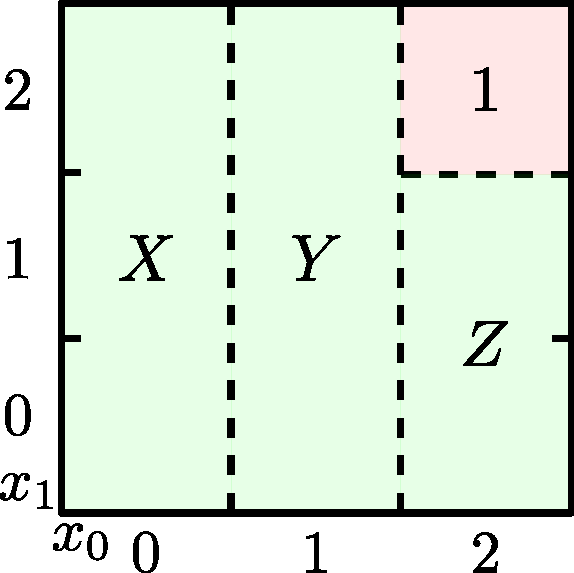
\includegraphics[scale=0.45]{figs/pd_split_thermal.pdf}
    \caption{\textbf{Qutrit phase space regions for $W_{\rho_{\rm{S}} | \sigma}(\x)$.}
    Here, the negative component of the magic state overlaps the Wigner distribution of $|0\>$. The rescaled distribution attains a single value in each of the four regions, proportional to the value depicted in the region, see~\cref{eq:bmw_rescaled}.
    }
    \label{fig:pd_split}
\end{figure}

The component values and multiplicities of the relevant distributions in the four distinct regions are summarised by the following component and multiplicity vectors,
\begin{align}
	\bmw(\rho_{\rm{S}}) &\coloneqq (-v, u, u, u), \\
		\bmm &\coloneqq (1,2,3,3), \\
	\bmw(\sigma) &\coloneqq \frac{1}{3\Z} \left( e^{-\beta E_0}, e^{-\beta E_0}, e^{-\beta E_1}, e^{-\beta E_2} \right), \\
	\bmw(\rho_{\rm{S}} | \sigma) &\coloneqq 3\Z \left( -v e^{\beta E_0}, u e^{\beta E_0}, u e^{\beta E_1}, u e^{\beta E_2} \right). \label{eq:bmw_rescaled}
\end{align}

Using this notation, the values and multiplicities of the $n$--copy distribution $\bmw(\rho^{\otimes n}_S |\sigma^{\otimes n})$ are computed in~\cref{lem:ncopycomponents} in~\cref{app:cmpairs}. The values are denoted by $w(\rho_{\rm{S}} | \sigma)_{ijk}$ with associated multiplicity $m_{ijk}$. The indices $i,j,k$ are non-negative integers and obey the constraint $\alpha \coloneqq i+j+k \leq n$.
The $n$--copy multiplicity is given by
\begin{equation}
	m_{ijk} = \frac{n!}{i!j!k!(n-\alpha)!} 2^i 3^j 3^k,
\end{equation}
while the distribution values are given by
\begin{align}\label{eq:ncopy_w_rescaled}
	w(\rho_{\rm{S}} | \sigma)_{ijk} &= (3\Z)^{n} (-v)^{n-\alpha} u^{\alpha} e^{\beta (n-\alpha)E_s} e^{\beta ( i E_0 + j E_1 + k E_2 )},
\end{align}
where we have also computed the unscaled components
\begin{align}
	w(\rho_{\rm{S}})_{ijk} &= (-v)^{n-\alpha} u^{\alpha}, \label{eq:ncopy_wrho}\\
	w(\sigma)_{ijk} &= (3\Z)^{-n} e^{-\beta (n-\alpha)E_s} e^{-\beta ( i E_0 + j E_1 + k E_2 )}. \label{eq:ncopy_wsigma}
\end{align}

In order to construct the $n$--copy Lorenz curve $\lc{\rho_{\rm{S}}^{\otimes n}}{\sigma^{\otimes n}}$ we need to order the components of the distribution, $w(\rho_{\rm{S}} | \sigma)_{ijk}$ in decreasing order.
In particular, to find the coordinates of the first elbow $(x_0, L_0)$, we need to evaluate the maximum component,
\begin{align}
	&w(\rho_{\rm{S}} | \sigma)_{\rm{max}} \coloneqq (3\Z)^{n}\times \nonumber\\
	&\max\limits_{i,j,k}\Big\{ (-v)^{n-\alpha} u^{\alpha} e^{\beta (n-\alpha)E_s} e^{\beta ( i E_0 + j E_1 + k E_2 )} \Big\}, \label{eq:max_slope}
\end{align}
where $0 \leq i,j,k \leq n$ and $\alpha \coloneqq i+j+k \leq n$.
For $0 \leq \epsilon \leq 3/7$, we have $v \geq u$. Since we assume that $n$ is even, we need the sum $\alpha = i+j+k$ to be even too, so that the expression is positive. 

Given an even value for $\alpha$, the term $v^{n-\alpha} u^{\alpha} e^{-\beta (n-\alpha)E_s}$ is fixed, so the expression is maximised by setting the coefficient of the highest energy $E_{\rm{max}}$ equal to $\alpha$.
Hence, we have
\begin{align}
	&w(\rho_{\rm{S}} | \sigma)_{\rm{max}} = \nonumber\\
	&(3\Z)^{n} v^n e^{n\beta E_s}\max\limits_{\substack{\alpha = 0,2, \\ \dots,n-2,n}}{\Big\{ \left( \frac{u}{v} e^{\beta (E_{\rm{max}} - E_s)} \right)^{\alpha} \Big\}}.
\end{align}
If the expression $\frac{u(\epsilon)}{v(\epsilon)} e^{\beta (E_{\rm{max}} - E_s)}$ is less than $1$ then the maximum occurs at $\alpha=0$, otherwise it occurs at $\alpha = n$. For a fixed stabilizer state $\sigma$, this transition is determined by the value of the depolarising noise parameter $\epsilon$ of the noisy magic state. The transition occurs at $\epsilon = \epsilon_\star$ where
\begin{equation}\label{eq:noise_transition}
	\frac{u(\epsilon_\star)}{v(\epsilon_\star)} e^{\beta (E_{\rm{max}} - E_s)} = \frac{3-\epsilon_\star}{6-8\epsilon_\star} e^{\beta (E_{\rm{max}} - E_s)} = 1.
\end{equation}
If $E_{\rm{max}} = E_s$, namely if the state negativity lies in the same phase space region as the highest energy, this threshold is constant in temperature and given by $\epsilon_{\star} = 3/7$. However, the condition that $\epsilon_\star \ge 0$ also implies a constraint on the effective temperature of the stabilizer state. Specifically, there is a threshold temperature value $\beta_\star$ given by
\begin{equation}
	\beta_{\star} \coloneqq \frac{1}{E_{\rm{max}} - E_s} \ln2,
\end{equation}
such that for the regime $0 \leq \beta \leq \beta_\star$ a transition noise level $\epsilon_\star$ exists, and for $\beta > \beta_\star$ no such transition exists, so we choose $\epsilon_\star = 0$. 
Therefore, the transition value for the noise is given by
\begin{equation}
	\epsilon_{\star}(\beta) \coloneqq 
	\begin{cases}
		3 - \dfrac{18}{8-2^{\beta/\beta_\star}}, &\text{ for } \beta \leq \beta_\star \\
		0, &\text{ for } \beta > \beta_\star.
	\end{cases}
\end{equation}
The quantity $w(\rho_{\rm{S}} | \sigma)_{\rm{max}}$ is now given by
\begin{equation*}
w(\rho_{\rm{S}} | \sigma)_{\rm{max}} =
	\begin{cases}
		(3\Z)^{n} v^n e^{n\beta E_s}, &\mbox{if }\epsilon \leq \epsilon_{\star},\ \hspace{3pt}\rm{(C1)}\\
		(3\Z)^{n} u^n e^{n\beta E_{\rm{max}}}, &\mbox{if }\epsilon > \epsilon_{\star}.\ \hspace{5pt}\rm{(C2)} 
	\end{cases}
\end{equation*}
Case $\rm{(C1)}$ corresponds to $(i,j,k) = (0,0,0)$, so the multiplicity is $m_{000} = 1$, while
Case $\rm{(C2)}$ corresponds to
\begin{equation}
	(i,j,k) = 
	\begin{cases}
	(0,n,0), &\text{if } E_{\rm{max}} = E_1, \\
	(0,0,n), &\text{if } E_{\rm{max}} = E_2,
	\end{cases}
\end{equation}
so the multiplicity in both cases is $3^n$.

Using that $F = -\beta^{-1} \log \Z$, the first elbow coordinates in the two cases are now given by
\begin{equation}\label{eq:first_elb_coords}
	(x_0, L_0) =
	\begin{cases}
		\left(\frac{1}{3^n} e^{-n\beta (E_s - F)}, v^n \right), &\epsilon \leq \epsilon_\star \vspace{10pt}\\
		\left( e^{-n\beta (E_{\rm{max}}-F)}, (3u)^n \right). &\epsilon > \epsilon_\star
	\end{cases}
\end{equation}
Similarly, considering the output magic state with respect to state $\sigma'$, the image of equilibrium state $\sigma$ under the magic protocol, we get output Lorenz curve coordinates,
\begin{equation}\label{eq:transformed_first_elb_coords}
	(x'_0, L'_0) =
	\begin{cases}
		\left(\frac{1}{3^{n'}} e^{-n\beta (E'_s - F')}, v(\epsilon')^{n'} \right), &\epsilon' \leq \epsilon'_\star \vspace{10pt}\\
		\left( e^{-n'\beta (E'_{\rm{max}}\hspace{-2.5pt}-F')}, (3u(\epsilon'))^{n'} \right), &\epsilon' > \epsilon'_\star
	\end{cases}
\end{equation}
There are four combinations of coordinates, depending on the noise parameters $\epsilon, \epsilon'$ for the input and output states.
In each of these combinations, we simply use the first elbow constraint, as described in~\cref{app:elb_constraints}, which leads to the bounds in the statement of the theorem.
%\begin{enumerate}
%	\item $\rm{(C1)} \rightarrow \rm{(C1)}$ if $E_{\rm{max}} = E_s$ or $E_{\rm{max}} > E_s$, $\beta < \beta_{\star}$ and $\epsilon' < \epsilon  \leq \epsilon_{\star}$.
%	\item $\rm{(C2)} \rightarrow \rm{(C1)}$ if $E_{\rm{max}} > E_s$, $\beta < \beta_{\star}$ and $\epsilon' \leq \epsilon_{\star} < \epsilon$.
%	\item $\rm{(C2)} \rightarrow \rm{(C2)}$ if $E_{\rm{max}} > E_s$, $\beta < \beta_{\star}$ and $\epsilon_{\star} \leq \epsilon' < \epsilon$ or $E_{\rm{max}} > E_s$, $\beta \geq \beta_{\star}$.
%\end{enumerate}
%The scenario $\rm{(C1)} \rightarrow \rm{(C2)}$ is not considered as it would correspond to $\epsilon \leq \epsilon_\star < \epsilon'$, which would imply that the output magic state is noisier than the input state.
%Substituting $\epsilon' = 0$ into these expressions leads to the stated distillation bounds.

\end{proof}



\subsection{Lower magic bounds via majorisation}
\label{sec:lower_bounds}

\ddd{[Initial text. To be edited.]}
We have described how relative majorization can be used to establish upper bounds on magic distillation protocols that take into account additional physics of the system. Given this, one might wonder if this approach could also provide \emph{lower bounds} for distillation protocols. Now, in contrast to the upper bounds, it is necessary to include the symplectic constraints on the phase space into the majorization relations.

  For example, the Clifford group action on a quantum system corresponds to the action of the affine symplectic group on the discrete phase space. Therefore, any convex mixture of Clifford unitaries will correpond to a convex mixture of these group actions. From the Hardy-Littlewood theorem, we know that traditional majorization is obtained from convex mixtures of arbitrary permutations. However this has been generalised to convex mixtures of elements of a group $G$ that acts on vectors. This $G$--majorization has been studied in the classical literature and a range of results are known about it. For example, if $G$ is a finite reflection group then the $G$--majorization pre-order is described by a finite list of conditions, just as happens for the full majorization ordering. One route is therefore to consider reflection sub-groups of the affine symplectic group, for which the majorization relation reduces to a finite set of conditions. This would therefore provide concrete lower bounds on distillation rates.
  
  The topic of $G$--majorization has been extensively studied, but to our knowledge there hasn't been work on relative $G$--majorization. This would correspond to transformations that are \emph{not} unital, but still respect the symplectic structure. Physically, this regime would correspond to a form of thermo-majorization obtained from looking at the action of the Clifford group at a micro-canonical level, and then reducing to a small subsystem. While this seems like a painful thing to consider, there is motivation for this beyond the aim of constructing lower bounds for magic protocols: in the case of statistical mechanics on a phase space this is precisely the situation, albeit in the continuum limit. Statistical mechanics of actual systems obey Hamiltonian dynamics and so automatically respect a symplectic form. Therefore the pre-order of statistical mechanical states with respect to phase space dynamics preserving a Gibbs state must correspond to a symplectic thermo-majorization condition. Of course, technical features arise in the continuum limit when considering distributions on an unbounded phase space, but this could be remedied by either considering a compact phase space (e.g. for a particle on a ring) or by first studying the discrete case.

%%%%%%%%%%%%%%%%%%%%%%%%%%%%%%%%%%%%%%%%
%
%\section{Fragments in general resource theories}
%\label{sec:general_resources}
%
%\nick{Add from notes}
%
%So far we have introduced the notion of $\sigma$--fragments for any resource theory of magic. 
%In this section we briefly generalise this concept to arbitrary resource theories and explain precisely how it connects with resource monotones. 
%The busy reader more focussed on magic may skip this section.
%
%State convertibility within a given resource theory is often a hard question to address due to intricacies of the theory structure.
%In general, the structure of a theory $\R$ is described by a pre-order $\prec_\R$ and usually resource monotones are employed to reduce this structure into a simple real number ordering.
%The subdivisions of magic theories into $\sigma$--fragments suggests a new approach towards investigating state convertibility which retains more structure of the original theory than a measure can.
%
%Monotones reduce the structure of the resource theory $\R$ to a \emph{total} order on the real numbers.
%Therefore, two states, even if incomparable in $\R$, are always mapped onto ordered real numbers.
%We now generalise this idea of a theory projection that preserves comparability between states. 
%\begin{definition}[\textbf{Covariant projection}]\label{def:covproj}
%Let $\R = (\F, \O)$ be a resource theory with pre-order $\prec_\R$. 
%Then a \emph{covariant resource projection} of $\R$ to a resource theory $\R'$ with pre-order $\prec_{\R'}$, is a pair of mappings $(\Pi_s, \Pi_o)$, where $\Pi_s$ maps quantum states in $\R$ to quantum states in $\R'$, and $\Pi_o$ maps free operations in $\R$ to free operations in $\R'$. 
%Moreover, these obey
%	\begin{enumerate}
%        \item $\Pis(\rho_1) \prec_{\R'} \Pis(\rho_2)$ whenever $\rho_1 \prec_\R \rho_2$;
%        \item $\Pio(\E) = \Pio(\E_1) \circ \Pio(\E_2)$ whenever $\E = \E_1 \circ \E_2$.
%    \end{enumerate}
%We call $\R'$ a \emph{covariant fragment} of $\R$.
%\end{definition}
%
%Resource monotones can now be clearly seen as a special case of covariant resource projections.
%\begin{proposition}[\textbf{Totally ordered covariant theories}]\label{thm:monoproj}
%	Any resource monotone $\M$ of a resource theory $\R$ is a covariant projection for which $\prec_{\R'}$ is a total order. 
%	Conversely, any such covariant projection corresponds to a resource monotone $\M$. 
%\end{proposition}
%\begin{proof}
%	Consider a monotone $\M$ in the context of a general resource theory $\R = (\F, \O)$.
%	State order is covariantly preserved due to the defining property of a monotone, where the pre-order $\prec_{\R'}$ is simply the total order $\leq$ on $\mathbb{R}$. 
%	
%	Operational composition is covariantly preserved when we simply choose $\Pio(\E) = 1_\times$, namely the `multiplication by 1' operation on real numbers. 
%	The definition of a resource monotone then automatically implies covariance.
%	
%	Conversely, given any covariant projection of $\R$ for which $\prec_{\R'}$ is a total order, we may map the totally ordered set of elements $\Pis(\rho)$ via an injective, non-decreasing function $f$ into $\mathbb{R}$. 
%	Then, $\M(\rho):=f(\Pi_s(\rho))$ provides a numerical value for each $\rho$ that obeys the definition of a monotone.
%	
%\end{proof}
%
%We can also view $\sigma$--fragments as an example of reducing the structure of a magic theory $\R$ to a subtheory with a tractable pre-order.
%However, states which are incomparable in $\R$ remain incomparable and conversions between states which are comparable in $\R$ may no longer be possible.
%\begin{definition}[\textbf{Contravariant projection}]\label{def:contraproj}
%	Let $\R = (\F, \O)$ be a resource theory with pre-order $\prec_\R$. 
%Then a \emph{contravariant resource projection} of $\R$ onto a resource theory $\R'$ with pre-order $\prec_{\R'}$, is a pair of mappings $(\Pi_s, \Pi_o)$, where $\Pi_s$ maps quantum states in $\R$ onto quantum states in $\R'$, and $\Pi_o$ maps free operations in $\R$ onto free operations in $\R'$. 
%Moreover, these obey
%	\begin{enumerate}
%        \item $\rho_1 \prec_\R \rho_2$ whenever $\Pis(\rho_1) \prec_{\R'} \Pis(\rho_2)$;
%        \item $\E = \E_1 \circ \E_2$ whenever $\Pio(\E) = \Pio(\E_1) \circ \Pio(\E_2)$.
%    \end{enumerate}
%We call $\R'$ a \emph{contravariant fragment} of $\R$.
%\end{definition}
%The use of covariant and contravariant in~\cref{def:covproj,def:contraproj} refers to the direction of implication between the two pre-orders and operation compositions\footnote{Note that strictly these are not projections in the sense of $\Pi^2 = \Pi$, but are instead morphisms. 
%Here our use of the term projection is motivated by the idea that one one generally loses information about $\R$ under the mapping.}.
%
%%%%%%%%%%%%%%%%%%%%%%%%%%%%%%%%%%%%%%%%%


\section{Outlook}
\label{sec:outlook}

In this work we have looked at magic through the lens of thermodynamics. Specifically, we find that it can be viewed as a strictly non-classical form of non-equilibrium free energy. 

Our work also raises a fundamental question that is also of interest in statistical mechanics. Specifically: what are the majorization conditions that respect the symplectic structure of phase space?

%%%%%%%%%%%%%%%%%%%%%%%%%%%%%%%%%%%%%%%%

\bibliography{bib}
%\bibliographystyle{apsrev4-2}

%%%%%%%%%%%%%%%%%%%%%%%%%%%%%%%%%%%%%%%%

\appendix
\section{Properties of majorization}
\label{app:major}

\subsection{Equivalent conditions for majorization}

\begin{theorem}
Given $\bmx, \bmy, \bmd \in \mathbb{R}^n$, such that the components of $\bmd$ are positive, the following statements are equivalent:
 \begin{enumerate}
	\item[(TM1)] $\bmx \prec_{\bmd} \bmy$;
	\item[(TM2)] $\Gamma_{\bmd}({\bmx}) \prec \Gamma_{\bmd}({\bmy})$;
	\item[(TM3)]\label{en:tm3} $\sum\limits_{i=1}^n \abs{x_i - t d_i} \leq \sum\limits_{i=1}^n \abs{y_i - t d_i}$ for all $t \in \mathbb{R}$;
	\item[(TM4)] $\sum\limits_{i=1}^n (x_i - t d_i)^+ \leq \sum\limits_{i=1}^n (y_i - t d_i)^+$ for all $t \in \mathbb{R}$ and $\sum\limits_{i=1}^n x_i = \sum\limits_{i=1}^n y_i$;
	\item[(TM5)] $\forall k, L_{\bmx|\bmd}(k) \leq L_{\bmy|\bmd}(k)$ and $L_{\bmx|\bmd}(k=n) = L_{\bmy|\bmd}(k=n)$.
 \end{enumerate}
\end{theorem}
\begin{proof}
    \begin{enumerate}
        \item[1$\leftrightarrow2$]
        Suppose now there exists a stochastic $S$ such that $\bmx = S\bmy$ with $\bmd = S\bmd$ and let $B = \Gamma_{\bmd} \circ S \circ \Gamma_{\bmd}^{-1}$.
        $B$ is a $D$-dimensional bistochastic matrix, since composition of stochastic matrices is stochastic and $(\Gamma_{\bmd} \circ S \circ \Gamma_{\bmd}^{-1}) (\frac{1}{D}\bm{1}) = (\Gamma_{\bmd} \circ S) (\bm{d}) = \Gamma_{\bmd}(\bm{d}) = \frac{1}{D}\bm{1}$. Then, $B$ maps $\Gamma_{\bmd}({\bmy})$ to $\Gamma_{\bmd}({\bmx})$.
        Conversely, given $B$, let $S = \Gamma_{\bmd}^{-1} \circ B \circ \Gamma_{\bmd}$.
        Similarly, $S$ is the stochastic matrix that preserves $\bmd$ and maps $\bmy$ to $\bmx$.
        \item[$2\leftrightarrow3$]\hspace{-5pt}, $2\leftrightarrow4$, $2\leftrightarrow5$ These three statement are equivalent to \nick{blah} respectively for the embedded vectors $\Gamma_{\bmd}({\bmx}), \Gamma_{\bmd}({\bmy})$.
        This is clear by rewriting
        \begin{align}
            \sum\limits_{i=1}^n \abs{x_i - t d_i} &= \sum\limits_{i=1}^n d_i \abs{\frac{x_i}{d_i} - t} = \sum\limits_{i=1}^D \abs{\Gamma_{\bmd}(\bmx)_i - t}, \\
            \sum\limits_{i=1}^n (x_i - t d_i)^+ &= \sum\limits_{i=1}^D (\Gamma_{\bmd}(\bmx)_i - t)^+, \\
            L_{\bmx|\bmd}(k) &= L_{\Gamma_{\bmd}(\bmx)}(k'), \\
            \text{with}\ k&=1,\dots,n\ \text{and}\ k'=1,\dots,D \nonumber
        \end{align} 
        and similarly for the right hand side.
    \end{enumerate}
\end{proof}

\subsection{Mana properties}
Mana monotonicity can be directly seen due to statement~\ref{en:tm3} in~\cref{thm:dmajor} for $t=0$.
Furthermore, mana is additive due to the multiplicative property~\ref{en:w4} of~\cref{thm:wstate}.

%%%

\section{Properties of the Wigner distribution}
\label{app:wigner}

Here we present important properties of the Wigner distribution that are used throughout the paper.

\begin{proposition}\label{thm:wstate}
    The Wigner distribution of a state $\rho$ is
    \begin{enumerate}%[label=\enlabel{W}{\arabic*}]
        \item\label{en:w1} Real valued: $\W{\rho} \in \mathbb{R}^{d^2}$;
        \item\label{en:w2} Normalised: $\sum_{\bmz \in \pd} \W[\bmz]{\rho}=1$;
        \item\label{en:w3} Bounded: $\abs{\W[\bmx]{\rho}} \leq \frac{1}{d}$.
        \item\label{en:w4} Additive under mixing:
        
        $\W[\bmx]{\sum_i p_i \rho_i} = \sum\limits_i p_i \W[\bmx]{\rho_i}$;
        \item\label{en:w5} Multiplicative under tensor products: 
        
        $\W[\bmx_A \oplus \bmx_B]{\rho_A \otimes \rho_B} = \W[\bmx_A]{\rho_A}\W[\bmx_B]{\rho_B}$.
	\end{enumerate}
\end{proposition}
A distribution satisfying the first three properties does not necessarily correspond to a positive semi-definite state.

\begin{proposition}
    \label{thm:wchannel}
    The Wigner distribution of a $\cptp$ operation $\E: \cal{B}(\hd[d_A]) \mapsto \cal{B}(\hd[d_B])$ is:
    \begin{enumerate}
        \item\label{en:wo1} Real-valued: $\W[\bmy|\bmx]{\E} \in \mathbb{R}$;
        \item\label{en:wo2} Normalised: $\sum_{\bmz \in \pd[d_B]} \W[\bmz|\bmx]{\E} = 1$ for any $\bmx \in \pd[d_A]$;
        \item\label{en:wo3} Bounded: $\abs{\W[\bmy|\bmx]{\E}} \leq \frac{d_A}{d_B}$;
	    \item\label{en:wo4} \nick{Transitive}: $\W[\bmy]{\E(\rho)} = \sum_{\bmz \in \pd[d_A]} \W[\bmy|\bmz]{\E} \W[\bmz]{\rho}$ for any $\bmy \in \pd[d_B]$.
    \end{enumerate}
\end{proposition}
If $d_A = d_B$, and in particular if operation $\E$ maps a Hilbert space onto itself, then the stochasticity condition $\abs{\W[\bmy|\bmx]{\E}} \leq 1$ is satisfied.

\end{document}